\documentclass[11pt]{article}

\usepackage{amssymb,amsmath,amsfonts,amsthm}
\usepackage{latexsym}
\usepackage{graphics}
\usepackage{indentfirst}
\usepackage{lmodern}
\usepackage{hyperref}
\usepackage{mathrsfs}
\usepackage{array}
\usepackage{mathtools}
\usepackage{graphicx}
\usepackage{setspace}
\usepackage{enumerate}
\usepackage{tikz}
\usepackage{url,color}
\usepackage{xcolor}
\usepackage{chngcntr}
\usepackage{multicol}
\usepackage{comment}
\usepackage{float}
\usepackage{algpseudocode}
\usepackage{subcaption}
\usepackage[ruled]{algorithm2e}
\usepackage{booktabs}
\usepackage{caption}
\usepackage[letterpaper,margin=2cm,top=2.5cm,bottom=2.5cm]{geometry}

\AtBeginEnvironment{algorithm}{\setstretch{1.2}}

\hypersetup{colorlinks=true,citecolor=blue,linkcolor=blue,urlcolor=blue}

%%%%%%%%%%%%%%%%%%%%%%%%%%%%%%%%%%%%%%%%%%%%%%%%%%%%%%%%%%
%% Theorem environments
%%%%%%%%%%%%%%%%%%%%%%%%%%%%%%%%%%%%%%%%%%%%%%%%%%%%%%%%%%
\newtheorem{theorem}{Theorem}[section]
\newtheorem{lemma}{Lemma}[section]
\newtheorem{proposition}{Proposition}[section]
\newtheorem{corollary}{Corollary}[section]
\newtheorem{remark}{Remark}[section]
\newtheorem{definition}{Definition}[section]

%%%%%%%%%%%%%%%%%%%%%%%%%%%%%%%%%%%%%%%%%%%%%%%%%%%%%%%%%%
%% Math shorthands
%%%%%%%%%%%%%%%%%%%%%%%%%%%%%%%%%%%%%%%%%%%%%%%%%%%%%%%%%%
\newcommand{\N}{\mathbb{N}}
\newcommand{\Z}{\mathbb{Z}}
\newcommand{\E}{\mathbb{E}}
\newcommand{\R}{\mathbb{R}}
\newcommand{\norm}[1]{\left\lVert#1\right\rVert}
\newcommand{\todo}[1]{\textcolor{red}{[#1]}}

\allowdisplaybreaks

%%%%%%%%%%%%%%%%%%%%%%%%%%%%%%%%%%%%%%%%%%%%%%%%%%%%%%%%%%
%% Title, authors, abstract
%%%%%%%%%%%%%%%%%%%%%%%%%%%%%%%%%%%%%%%%%%%%%%%%%%%%%%%%%%

\title{Diffusion Proposals for Redistricting Markov Chains}

\author{Alaittin K\i rt\i \c{s}o\u{g}lu \\
        \small Department of Applied Mathematics, Illinois Institute of Technology \\
        \small Chicago, IL 60616 \\
        \small \texttt{kirtisoglu@hawk.iit.edu}}

\date{\today}

\begin{document}

\maketitle

\begin{abstract}
Recombination (ReCom) chains are the standard Markov chain Monte Carlo
tool for sampling redistricting plans, and they are routinely run under
a Metropolis filter that nominally targets a compactness-tempered
distribution. We introduce a proposal built from graph diffusion. One
convex energy on the merged pair of districts, a kernel-weighted
Laplacian smoothness term plus a fidelity term that anchors each move to
the current plan, is minimized under global population balance and
rounded at random. The diffusion view yields a small theory of the
proposal: its optimum is a single linear solve whenever balance is
slack, the expected number of units a proposal moves is an explicit
high-pass filter norm with a provable ceiling, and mobility is governed
by feasibility rather than by the Metropolis ratio, which gives a tuning
rule. Correcting the rounding with an exact Metropolis--Hastings step
gives, to our knowledge, the first optimization-based redistricting
proposal with a detailed-balance proof. Mixed with the forest-lifted
recombination move Metropolized to the same target, it yields a
reversible sampler for kernel-weighted compactness distributions,
validated against enumerated targets. On Iowa it roughly doubles the
effective samples per second of the forest move alone under perimeter
and density targets, and adds nothing on the spanning-tree-weighted
measure. The reason is structural, and we measure it: the tree move is
an independence sampler from the untempered spanning-tree measure, so
its acceptance decays exponentially with the size of the merged pair
under any compactness-tempered target, while the local move has a dial
for the same effect. On an enumerated test bed we also show, at the
level of distributions, that plain and tempered ReCom do not sample
their nominal target and sit close to the spanning-tree-weighted
measure.
\end{abstract}

%% DRAFT v2, 2026-10-22. Rebuilt from paper.tex after the Forest ReCom kill
%% test and the scaling experiment. Precinct-scale sections are left as
%% placeholders marked \todo.

%════════════════════════════════════════════════════════════════════════════════
\section{Introduction}\label{sec:intro}
%════════════════════════════════════════════════════════════════════════════════

\subsection{The redistricting problem and ReCom's role}\label{sec:intro-problem}

Political redistricting seeks a partition of a geographic region into
electoral districts satisfying legal, demographic, and geometric
requirements, namely contiguity, population balance, compactness, and
preservation of communities of interest. Computational approaches model
the problem on the dual adjacency graph $G = (V,E)$ of geographic units
(precincts, census blocks, counties). A valid $k$-district plan is a
partition
\[
  P = \{V_1, \ldots, V_k\}, \qquad \bigsqcup_{i=1}^k V_i = V,
\]
where each $G[V_i]$ is connected and the populations $p(V_i)$ are
approximately equal. Let $\mathcal{P}_k(G)$ denote the space of valid
$k$-district plans. The cardinality of $\mathcal{P}_k(G)$ is enormous.
Even four congressional districts over the 99 counties of Iowa admit
roughly $10^{24}$ plans~\cite{fifield2020essential}.

Markov chain Monte Carlo (MCMC) has become the standard tool for
sampling $\mathcal{P}_k(G)$. Early flip chains modify a single
precinct's assignment per step~\cite{fifield2020automated} and mix
slowly. The Recombination (ReCom) algorithm of DeFord, Duchin, and
Solomon~\cite{deford2021recombination} performs multi-precinct updates
by merging two adjacent districts, sampling a uniform random spanning
tree of the merged subgraph, and cutting an edge to recover a balanced
bipartition. ReCom dramatically improved the mixing efficiency of
redistricting MCMC and is now the workhorse of the field, with
reversible~\cite{cannon2022spanning}, forest-lifted~\cite{autry2023metropolized}
and multi-scale~\cite{autry2020multiscale} extensions.

\textbf{ReCom's blind spot.} The uniform spanning-tree split treats
every edge of the merged subgraph identically. The proposed
bipartition is determined by the topology of the merged subgraph
alone. Real geography is not topology-only. Shared boundary
length, population density, demographic similarity, and
administrative boundaries all carry signal that could shape the
proposed split. Practitioners have felt this. County-weighted
trees~\cite{clelland2022colorado} and GerryChain's region-aware
surcharges~\cite{gerrychain2024} inject indicator-based edge weights
into the tree draw, and SpecReCom~\cite{davies2025spectral} replaces
the tree with a Fiedler-vector cut of a randomly weighted Laplacian.
But these mechanisms are restricted (region indicators, hard-coded
county kernels, or no kernel at all), none includes a
locality-preserving fidelity term, and, as their authors
acknowledge, each shifts the chain's stationary distribution in
an uncharacterized, uncorrected way.

\textbf{A second blind spot, which this paper measures.} Even the
exact versions of the tree move, which Metropolize it to a stated
target, propose from one fixed law, the spanning-tree measure on
balanced splits of the merged pair. Whenever the target a practitioner
wants is not close to that law, for instance a compactness-tempered
target or a geography-weighted one, the Metropolis step has to undo
the mismatch on every proposal, and the mismatch grows with the size
of the merged pair. We show that the resulting acceptance decays
exponentially in the pair size, which is the structural reason an
exact sampler for such targets needs a second kind of move.

\subsection{Contribution}\label{sec:intro-contribution}

We introduce a diffusion proposal for ReCom-style MCMC and the exact
sampler built on it. The core object is a single Laplacian energy on
the merged-pair subgraph $H = G[V_i \cup V_j]$,
\begin{equation}\label{eq:core-energy}
  E(x) \;=\; \alpha\, x^\top L\, x \;+\; \beta\, \|x - x_0\|^2,
  \qquad
  (1 - \varepsilon)\bar p \;\le\; p^\top x \;\le\; (1+\varepsilon)\bar p,
\end{equation}
where $L$ is the kernel-weighted graph Laplacian of $H$, $x_0$ encodes
the current bipartition, and the balance constraint is anchored to the
global per-district ideal (Equation~\eqref{eq:balance-window}). The
Laplacian term $x^\top L x$ counts (or approximates) cut edges between
the two sides; the fidelity term $\|x - x_0\|^2$ penalizes deviation
from the current assignment, enforcing locality of each move. The
paper makes four contributions.

\begin{enumerate}
  \item \textbf{A diffusion proposal with a theory of its own
    behavior} (\S\ref{sec:qp-model}--\S\ref{sec:diffusion-theory}).
    The interior optimum of the energy is one implicit Euler step of
    the graph heat equation with timestep $\tau = \alpha/\beta$. We
    show that this step is a single linear solve whose output lies in
    the unit cube automatically, so the box constraints never bind
    and the proposal costs a linear solve whenever population balance
    is slack (Lemma~\ref{lem:row-stochastic}). Under single-shot
    Bernoulli rounding, the expected number of units a proposal moves
    is exactly the one-norm of a high-pass filter applied to the
    current split (Proposition~\ref{prop:move-size}). That quantity
    grows like twice the timestep times the pair's boundary for small
    timesteps and is bounded above by half the merged pair for any
    timestep (Corollary~\ref{cor:small-tau}). Given a feasible
    proposal the Metropolis step accepts it at least 98 percent of the
    time; the chain's stickiness is a feasibility effect with an
    interior optimum in $\tau$ (\S\ref{sec:mobility}), and its
    mobility is given to within counting noise by a two-swap law,
    Equation~\eqref{eq:mobility-law}.

  \item \textbf{An exactly reversible correction}
    (\S\ref{sec:qp-mh}). Correcting the rounding with an exact
    Metropolis--Hastings step yields Chain E, to our knowledge the
    first optimization-based redistricting proposal with a
    detailed-balance proof (Proposition~\ref{prop:qpmh-db}), stated
    on labeled plans, where the proposal map is a bijection. We
    verify the implemented kernel to machine precision on an
    enumerated fiber and show by a batch-means test that a
    million-step run's occupancy distribution is not distinguishable
    from the exact target (\S\ref{sec:exp-2x3}).

  \item \textbf{An exact sampler for kernel-weighted compactness
    targets, and a measurement of when its local component matters}
    (\S\ref{sec:hybrid}, \S\ref{sec:exp-hybrid}--\S\ref{sec:exp-scaling}).
    We lift Chain E to the spanning-forest state space and mix it with
    the forest-lifted recombination move of Autry et
    al.~\cite{autry2023metropolized}, Metropolized to an arbitrary
    kernel-weighted target. The mixture is verified to machine
    precision on an enumerated lifted fiber and against enumerated
    targets on 4\,006 plans. On Iowa, under a criterion fixed before
    the runs, the mixture gives $1.6$ to $2.3$ times the forest move's
    effective samples per second under perimeter and density targets
    on two seeds, and $0.8$ to $0.9$ times under the
    spanning-tree-weighted tempered measure. We then show why. The
    forest move is an independence sampler from the untempered
    spanning-tree measure on balanced splits; on $N \times N$ grids its
    acceptance at equilibrium falls like $e^{-0.24 N}$ under
    compactness-tempered targets, with or without tree weighting, while
    the per-proposal mismatch in its Hastings ratio grows in
    proportion to the boundary length. The local move loses
    acceptance with pair size too, but has a dial for it, the
    move-size law; the tree move has none.

  \item \textbf{A ground-truth calibration of what the ReCom family
    samples, at the level of distributions}
    (\S\ref{sec:exp-5x5}, \S\ref{sec:exp-iowa-calib}). On a fully
    enumerated $5 \times 5$ fiber we compute the spanning-tree-weighted
    measure for every state by the Matrix--Tree theorem and compare full
    empirical distributions against it and against the nominal tempered
    target, with sampling-noise floors at the effective sample size.
    The tempered chain's cut distribution is 220 floor standard
    deviations from its nominal target and close to, though
    distinguishable from, the tree-weighted tempered measure, while the
    exact chain is indistinguishable from the nominal target. On Iowa
    the exact sampler puts the nominal target's mean cut count near
    $88$ and the tree-weighted measure's at $41$, where tempered ReCom
    sits at $40$.
\end{enumerate}

\paragraph{Positioning.} The construction of Chain E, a deterministic
optimization that sets the parameters of a random proposal which is
then corrected exactly, has ancestors outside redistricting.
Randomize-then-optimize~\cite{bardsley2014randomize} samples
posteriors by perturbing and solving, and Zanella's informed
proposals~\cite{zanella2020informed} give the general theory of
locally balanced, target-aware proposals on discrete spaces. Chain E
is an instance of that program on the space of plans, and our
priority claim is scoped to redistricting accordingly. Within
redistricting, the known-target samplers, Metropolized forest
recombination~\cite{autry2023metropolized}, RevReCom, Cycle Walk,
Marked Edge Walk, and
BUD~\cite{cannon2022spanning,deford2025cycle,mcwhorter2025marked,
akitaya2026bud}, achieve computable transition probabilities by
lifting to spanning-forest state spaces, while Chain E achieves the
same property at the partition level; the two routes are
complementary, and the forest move is the global component of our
sampler. Bonsai sampling~\cite{clelland2026bonsai} draws independent
plans from a specified law without a chain and is the natural non-MCMC
comparison for any known-target method. \S\ref{sec:related} positions
the proposal against the weighted-tree, spectral, and matheuristic
lines.

\paragraph{Roadmap.}\label{sec:intro-roadmap}
\S\ref{sec:related} reviews related work and \S\ref{sec:background}
sets up notation. \S\ref{sec:model} develops the proposal, its
theory, the exact chain, and the sampler; \S\ref{sec:experiments}
reports the calibration, the convergence validation, the kill test
against the forest move, the scaling experiment, and the Iowa
calibration. Appendices hold hyperparameters, a partition-fiber
diagnostic, and a reproducibility checklist.

%════════════════════════════════════════════════════════════════════════════════
\section{Related work}\label{sec:related}
%════════════════════════════════════════════════════════════════════════════════

\paragraph{MCMC for redistricting.}\label{sec:related-mcmc}

Early MCMC for redistricting framed the problem as a graph cut and used
single-unit flip chains~\cite{fifield2020automated} or
Swendsen--Wang-style large-swap moves. Flip chains mix poorly and
produce highly irregular districts~\cite{deford2021recombination,
najt2024empirical}. ReCom~\cite{deford2021recombination} introduced
the spanning-tree merge-split move and is now standard. Extensions
include Multi-Scale Merge--Split~\cite{autry2020multiscale} preserving
nested communities (counties, precincts), Metropolized forest
recombination~\cite{autry2023metropolized}, Sequential Monte
Carlo~\cite{mccartan2023sequential} and its generalized
form~\cite{osullivan2026generalized}, whose repetition effects are
analyzed in~\cite{cannon2024repetition}, multiscale parallel
tempering~\cite{chuang2025multiscale}, and reversible
recombination~\cite{cannon2022spanning} targeting the canonical
spanning-tree distribution. The compactness-tempered target that
practitioners run under a Metropolis filter, and that we audit here,
originates in the North Carolina analyses of Herschlag et
al.~\cite{herschlag2020quantifying}. The 50-State Redistricting
Atlas~\cite{mccartan2022simulated} is the field's standard ensemble
benchmark. A consistent theme of the 2022--2026 literature is that a
sampler is only as defensible as its target.
RevReCom~\cite{cannon2022spanning}, Metropolized forest
recombination~\cite{autry2023metropolized}, the cycle
walk~\cite{deford2025cycle}, and the marked edge
walk~\cite{mcwhorter2025marked} all pay a structural price (lifted
state spaces, spanning-forest counting) precisely to keep transition
probabilities computable. On the theory side, Cannon, Pegden, and
Tucker-Foltz~\cite{cannon2024sampling} give a polynomial-time sampler
for the spanning-tree measure on balanced partitions of grids with a
constant number of districts, Gold~\cite{gold2026adversarial}
exhibits planar-grid configurations from which recombination needs
exponentially many expected steps to re-split, and mixing-time bounds
for the local chains used in practice remain open. Akitaya et
al.~\cite{akitaya2022reconfiguration} prove that deciding
reachability between balanced partitions under recombination is
PSPACE-complete when the district count and step size grow with the
graph.

\paragraph{Weighted and geography-aware proposals.}\label{sec:related-weighted}

Edge weighting inside the ReCom proposal is not new, and we position
our work against it explicitly. Clelland et
al.~\cite{clelland2022colorado} replace the proposal's edge-weighting
function with \emph{county-weighted trees} (intra-county edge
weights drawn from the uniform distribution $\mathcal{U}[0, w]$ for a
tunable scalar $w$) to reduce county splits in Colorado ensembles.
GerryChain's region-aware ReCom~\cite{gerrychain2024} implements the
same idea. User-specified surcharges are added to the randomized
Kruskal weights for edges crossing designated region boundaries.
Tapp~\cite{tapp2025compactness} modifies the ReCom tree-and-cut step
to improve shape-based compactness at the proposal level. In all
three, the weighting is an indicator- or attribute-indexed heuristic,
and (as their authors acknowledge) the induced stationary distribution
is uncharacterized and uncorrected. What the unweighted tree proposal
itself induces is better understood. Clelland et
al.~\cite{clelland2021compactness} measured ReCom ensembles on grids
and precinct graphs and found the sampling probability of a plan to
decay roughly exponentially in its cut length, and Procaccia and
Tucker-Foltz~\cite{procaccia2022compact} proved the underlying fact
that compact plans have many spanning trees. Tapp, Proebsting, and
Ramsay~\cite{tapp2025parameter} study how tolerance and
county-preservation settings move ReCom ensembles and propose
effective-sample-size diagnostics for them. Our calibration in
\S\ref{sec:exp-5x5} makes the first of these observations exact on an
enumerated fiber, at the level of full distributions, and our scaling
experiment in \S\ref{sec:exp-scaling} turns the second into a
statement about acceptance: the same exponential that makes compact
plans tree-rich is what an exact tree move has to pay, per proposal,
to target anything else. Conversely, the samplers with known targets
cited above handle only unweighted spanning-tree/forest measures or
other tree-count-based families. The gap this paper addresses sits at
the intersection, namely a proposal that accepts an \emph{arbitrary}
nonnegative edge kernel as a first-class input together with an exact
accept/reject step against a stated target (\S\ref{sec:qp-mh},
\S\ref{sec:hybrid}).

\paragraph{Optimization-based districting and matheuristics.}\label{sec:related-opt}

A parallel operations research (OR) literature treats districting as
exact optimization. Examples include the Hess model lineage,
column-generation and set-partitioning
formulations~\cite{gurnee2021fairmandering}, multilevel
multiobjective methods~\cite{swamy2023multiobjective},
contiguity-constrained MIPs~\cite{validi2022imposing}, and cut-edge
minimization solved to optimality at county/tract
scale~\cite{validi2022political}. Dobbs et al.~\cite{dobbs2024facilitating}
solve for minimal-change and midpoint plans under transfer distance to
reference plans exactly by mixed-integer programming. Between the
sampling and optimization families~\cite{becker2022redistricting},
hybrids are emerging. Short bursts~\cite{cannon2023voting} use ReCom
as a stochastic optimizer; Brous and Shmoys~\cite{brous2025recom}
replace the spanning-tree re-split with a Gurobi integer program
inside an accept-if-better local search for majority-minority
districts. The integer form of our energy, a convex MIQP refinement
inside a recombination chain, belongs to this matheuristic line; we
note in \S\ref{sec:disc-future} what we found when we evaluated it as
an optimizer, and do not pursue it here. The proximal term
$\beta\|x - x_0\|^2$ is the quadratic analogue of local
branching~\cite{fischetti2003local}, imposing a soft trust region
around the incumbent.

\paragraph{Spectral partitioning and diffuse-interface models.}\label{sec:related-spectral}

Spectral graph partitioning has a long history in image segmentation
and clustering~\cite{shi2000normalized}. In redistricting, the recent
SpecReCom of Davies, Job, Kampbell, Kim, and
Seo~\cite{davies2025spectral} (arXiv preprint, June 2025) replaces the
random spanning tree with a Fiedler-vector sign cut on a randomly
edge-weighted Laplacian of the merged pair, reporting roughly half the
cut edges of RevReCom on a $56 \times 56$ grid and a Colorado planar
graph. Plain SpecReCom sacrifices population balance, which their
BalSpecReCom variant partially restores. Diffuse-interface models
build on the Ginzburg--Landau (GL) functional, combining a smoothness
term with a fidelity term; the Chan--Vese model~\cite{chan2001active}
and Merriman--Bence--Osher (MBO) threshold dynamics implement this
iteratively. Bertozzi and collaborators~\cite{bertozzi2012diffuse,
merkurjev2013mbo} port the machinery to weighted graphs, where the
smoothness term becomes the Laplacian quadratic form $x^\top L x$ and
graph Tikhonov regularization~\cite{pilavci2021graph,shuman2013emerging}
recovers heat-kernel smoothing. Jacobs and Walch~\cite{jacobs2018pde}
brought threshold dynamics to redistricting before SpecReCom, using
volume-constrained MBO via auction dynamics~\cite{jacobs2018auction}
to generate compact equal-population maps. Theirs is a continuum PDE
approach, not a graph-kernel one, and it is not embedded in MCMC. To our
knowledge the present work is the first to use the \emph{graph} GL
lineage (kernel-weighted Laplacian smoothing plus fidelity) as a
proposal inside redistricting MCMC.

\paragraph{Cut minimization and discrete compactness.}\label{sec:related-cut}

The minimum graph cut~\cite{stoer1997simple,karger2000minimum} and its
balanced variants such as normalized cut~\cite{shi2000normalized} are
classical objectives. NP-hardness of balanced minimum
cut~\cite{wagner1993between} motivates continuous relaxations, of
which the Fiedler-vector cut and the Total Variation Isoperimetric
Profile~\cite{deford2019total} are two well-known examples. The cut
edge count $|\partial P|$ has been proposed as a discrete compactness
measure for redistricting~\cite{duchin2018discrete} and shown to
correlate well with classical geometric scores (Polsby--Popper, Reock)
while being more stable under unit refinement.

%════════════════════════════════════════════════════════════════════════════════
\section{Background: plans and ReCom}\label{sec:background}
%════════════════════════════════════════════════════════════════════════════════

\subsection{Dual graph and \texorpdfstring{$k$}{k}-district plans}\label{sec:background-graph}

Let $G = (V, E)$ be the dual graph of a state, with vertices
representing geographic units (precincts, census blocks, counties) and
edges encoding shared boundaries. Each vertex $v$ carries a population
$p_v \ge 0$ and may carry additional attributes (demographic vectors,
shapefile geometry). A \emph{$k$-district plan} is a partition
$P = \{V_1, \ldots, V_k\}$ of $V$ such that each induced subgraph
$G[V_i]$ is connected (\emph{contiguity}) and the populations satisfy
\begin{equation}\label{eq:pop-balance}
  (1 - \varepsilon)\bar p \;\le\; p(V_i) \;\le\; (1 + \varepsilon)\bar p,
  \qquad \bar p := \frac{p(V)}{k},
\end{equation}
for a tolerance $\varepsilon \in [0, 1)$. We write $\mathcal{P}_k(G; \varepsilon)$
for the set of valid plans. The \emph{cut edges} of a plan are
\[
  \partial P \;=\; \{(u,v) \in E : P(u) \ne P(v)\},
\]
and we call $|\partial P|$ the \emph{cut-edge count} of $P$. This
quantity is the discrete analog of the perimeter of the district
boundaries and serves as our primary compactness
metric~\cite{duchin2018discrete}. For a nonnegative edge kernel $w$ we
write $w(\partial P) = \sum_{e \in \partial P} w_e$ for the
\emph{weighted cut}.

\begin{figure}[htbp]
  \centering
  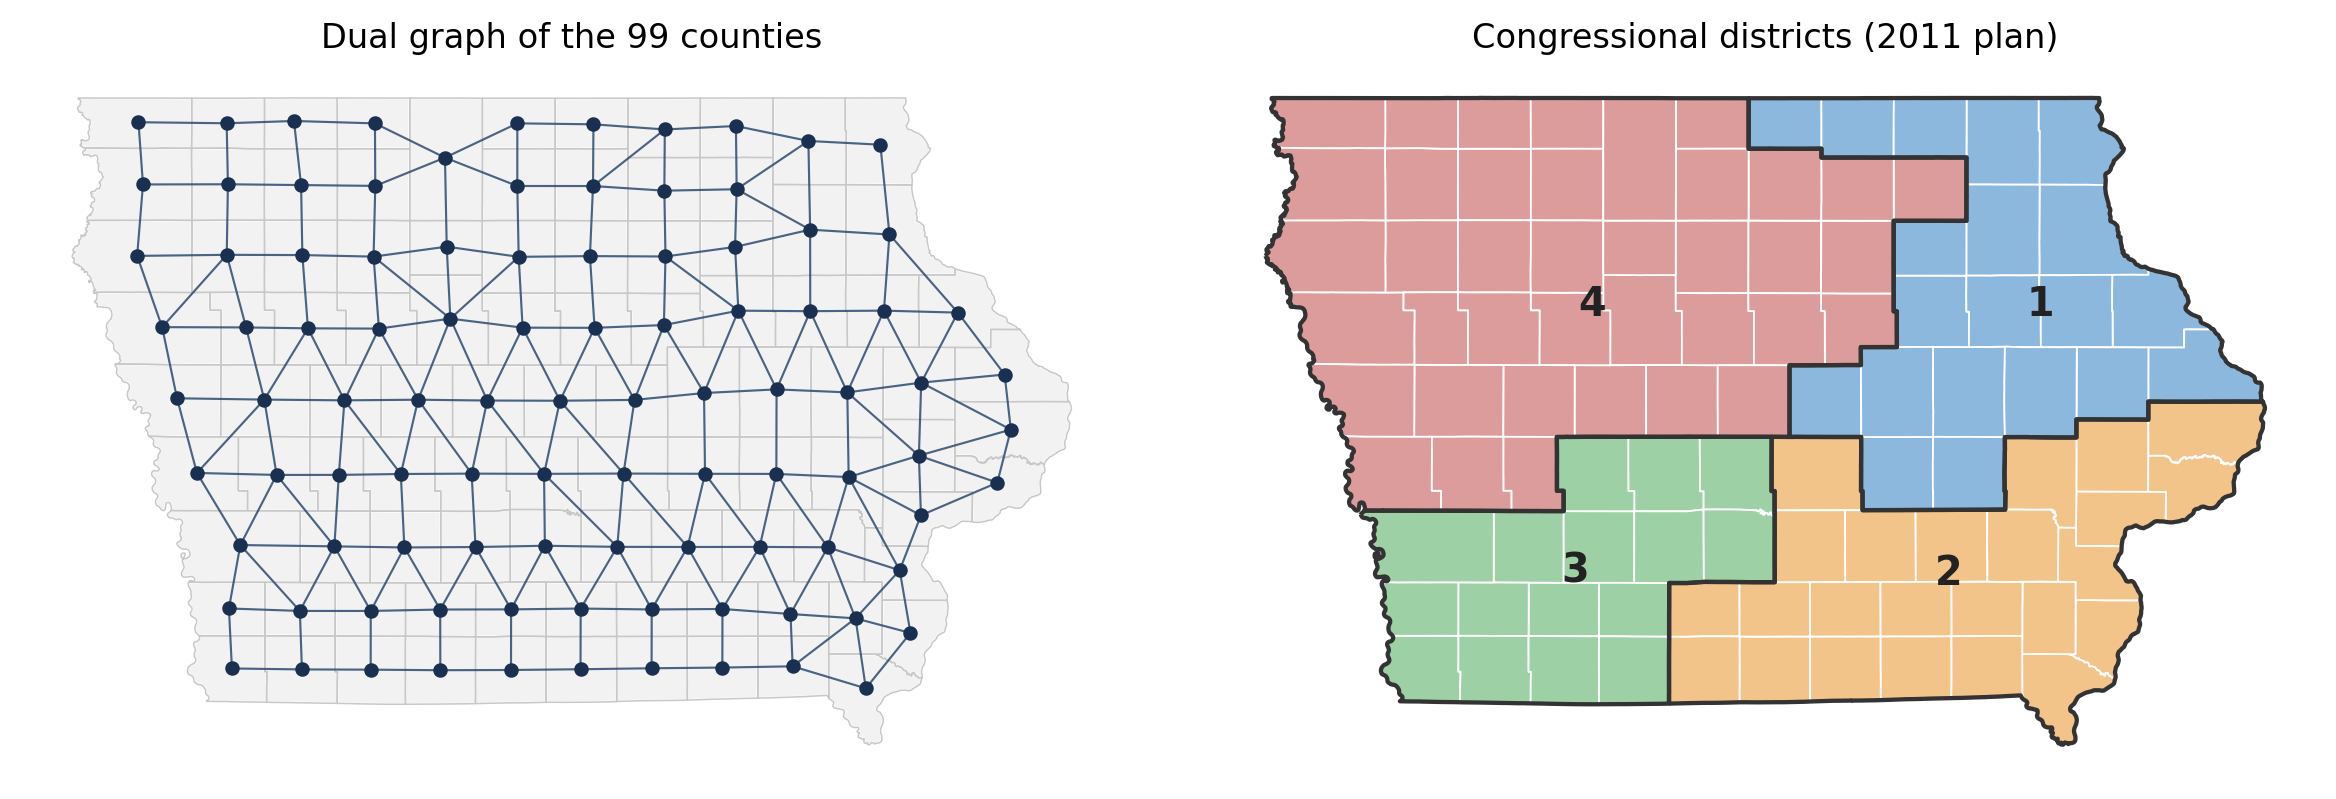
\includegraphics[width=0.5\textwidth]{fig/redistricting.png}
  \caption{The dual graph of Iowa's 99 counties (left) and the four
    congressional districts enacted after the 2010 census (right).
    Nodes sit at county centroids; two counties are joined by an edge
    when they share a boundary segment.}
  \label{fig:iowa-dual}
\end{figure}

\subsection{Recombination (ReCom)}\label{sec:background-recom}

Recombination~\cite{deford2021recombination} is a Markov chain on
$\mathcal{P}_k(G; \varepsilon)$ whose single step is given in Algorithm~\ref{alg:recom}.

\begin{algorithm}[H]
\caption{Vanilla ReCom step (Chain V)}\label{alg:recom}
\KwIn{Current plan $P$, dual graph $G$, balance tolerance $\varepsilon$.}
\KwOut{Next plan $P'$.}
Select two adjacent districts $V_i, V_j$ uniformly at random from boundary pairs;\\
Form the induced subgraph $H = G[V_i \cup V_j]$;\\
\Repeat{a cut $e^*$ exists yielding two $\varepsilon$-balanced components}{
  Sample a uniform random spanning tree $T$ of $H$ via Wilson's algorithm~\cite{wilson1996generating};\\
  Search edges of $T$ for a cut $e^*$ whose removal produces two $\varepsilon$-balanced components.
}
Define $V_i', V_j'$ as the two components of $T \setminus \{e^*\}$;\\
$P' \gets P$ with $V_i, V_j$ replaced by $V_i', V_j'$;\\
\Return $P'$.
\end{algorithm}

\noindent The tree-based proposal flips many precincts simultaneously
between $V_i$ and $V_j$ while preserving contiguity automatically (any
edge removal from a tree produces two connected components). This is
the key advantage over single-precinct flip chains, which traverse the
state space too slowly to be practically useful.

\textbf{Chains compared.} Table~\ref{tab:chains} lists the chains of
this paper.

\begin{table}[htbp]
\centering
\small
\begin{tabular}{llll}
\toprule
Chain & Method & Mechanism & Stationarity claim \\
\midrule
V & Vanilla ReCom~\cite{deford2021recombination} & spanning-tree split, always accept & unknown target \\
A & Tempered ReCom & ReCom + MH on cuts (symmetric-$q$) & approximate \\
E & QP-MH (this work, \S\ref{sec:qp-mh}) & QP + Bernoulli rounding + exact MH & \textbf{exact} \\
T & Partition-level tree move (\S\ref{sec:tree-partition}) & uniform tree, uniform edge, tree-count MH & \textbf{exact} \\
F & Forest move (\S\ref{sec:forest}) & forest-lifted ReCom, balanced edge, exact MH & \textbf{exact} \\
H & Hybrid (this work, \S\ref{sec:hybrid}) & mixture of F and lifted E, any kernel-weighted target & \textbf{exact} \\
\bottomrule
\end{tabular}
\caption{The chains compared in this paper. The last column is the
  chain's relationship to its stated target. Chains E, T, F and H carry
  exact Metropolis--Hastings corrections; Chain A relies on the
  symmetric-$q$ approximation (\S\ref{sec:qp-mh}) and Chain V has
  no stated target. Chain T is kept as the reference that explains
  Chain A and as the baseline of an earlier version of this work;
  Chain F is the baseline the sampler is judged against.}
\label{tab:chains}
\end{table}

Tempered ReCom uses a Metropolis--Hastings filter targeting
$\pi(P) \propto \exp(-\lambda |\partial P|)$ with the symmetric-$q$
approximation (treating the forward and reverse proposal probabilities
as equal); see Appendix~\ref{app:hyperparams} for the locked-in
$\lambda = 0.10$. All chains enforce the global
two-sided balance window of Equation~\eqref{eq:balance-window} on
every move; we note (\S\ref{sec:exp-balance}) that the raw GerryChain
\texttt{recom} proposal alone does not.

\paragraph{The proposal we replace.}\label{sec:background-weakness}
The tree-and-cut step is kernel-blind (\S\ref{sec:intro-problem}),
and the cut edge is chosen only after the tree is drawn, so the
proposal cannot anticipate the shape of the split. The diffusion
proposal of \S\ref{sec:model} replaces that step with a single convex
optimization of a kernel-weighted Laplacian energy plus a
locality-preserving fidelity term. The energy
$x^\top L\, x = \sum_{(u,v) \in E} w_{uv} (x_u - x_v)^2$ equals the
weighted cut count for binary $x$, so minimizing it directly
minimizes the discrete perimeter in the chosen kernel.

%════════════════════════════════════════════════════════════════════════════════
\section{The QP-diffusion model, its theory, and the sampler}\label{sec:model}
%════════════════════════════════════════════════════════════════════════════════

The energy~\eqref{eq:core-energy} has three ingredients: the kernel
that defines the Laplacian (\S\ref{sec:kernels}), the convex program
on the merged pair (\S\ref{sec:qp-model}, with its spectral form
\eqref{eq:freq-response}), and the balance window. The rest of the
section builds the chains on top of it.

\subsection{Locality kernels}\label{sec:kernels}

Choosing the edge weights $w_{ij}$ is the most important modeling
decision. The kernel determines what \emph{smoothness} means and
therefore controls how district boundaries move under the relaxation.
We restrict all weights to geographic neighbors,
\begin{equation}\label{eq:kernel-local}
  w_{ij} = 0 \quad \text{if } (v_i, v_j) \notin E,
\end{equation}
ensuring that diffusion operates only through geographic adjacency and
preventing long-range interactions that could produce disconnected
districts.

\paragraph{Uniform kernel ($k_{\mathrm{unif}}$).} $w_{ij} = 1$ for
every edge. The Laplacian $L$ is the combinatorial graph Laplacian;
$x^\top L x$ is exactly the cut edge count. In the $\beta \to 0^+$
limit the proposal approaches a balanced Fiedler-style split.

\paragraph{Perimeter kernel ($k_{\mathrm{perim}}$).} $w_{ij} = |\partial v_i \cap \partial v_j|$
(shared-boundary length). The Laplacian quadratic form $x^\top L x$
is then the \emph{geographic perimeter} of the partition, weighted by
boundary segment length. This kernel discourages fragmented districts
and favors boundaries that cut along short segments.

\paragraph{Density kernel ($k_{\mathrm{dens}}$).} Let $\rho_v$ denote
the population density at vertex $v$ (population per unit area). A
Gaussian density kernel
\[
  w_{ij} \;=\; |\partial v_i \cap \partial v_j| \cdot
  \exp\!\Bigl( -\frac{(\rho_i - \rho_j)^2}{\sigma^2} \Bigr)
\]
encourages cuts along sharp density gradients (urban--rural
boundaries) while preserving the topological role of shared boundary
length.

\paragraph{Demographic kernel ($k_{\mathrm{demog}}$).} Let
$d_v \in \R^m$ be a vector of demographic attributes. A Gaussian
similarity kernel $w_{ij} = \exp(-\|d_i - d_j\|^2 / \sigma^2)$
encourages communities of interest. We define this kernel for
completeness but do not use it in our experiments, and a caution
stronger than ``use as a soft regularizer'' is warranted. If the
attribute vector encodes race, a proposal that systematically shapes
district boundaries around racial similarity risks making race the
predominant districting criterion, which triggers strict scrutiny
under the \emph{Shaw v.\ Reno} line of racial-gerrymandering cases.
Any practical use of demographic kernels should be reviewed against
that doctrine, should document the kernel's weight relative to
race-neutral criteria, and is more defensible for attributes that are
legitimate districting factors in the jurisdiction (e.g., municipal
membership, communities of interest as defined by state law).

\paragraph{Composite kernels.} Linear combinations $w_{ij} = \sum_k a_k w_{ij}^{(k)}$
with $a_k \ge 0$ remain valid, since they preserve nonnegativity and locality.

\subsection{The convex QP}\label{sec:qp-model}

Let $H = G[V_i \cup V_j]$ be the merged subgraph of two adjacent
districts. Let $L_H$ be the kernel-weighted Laplacian of $H$, let
$x_0 \in \{0,1\}^{|V_H|}$ encode the current bipartition (1 for
vertices in $V_i$, 0 for vertices in $V_j$), and let $p$ be the
population vector restricted to $H$. Fix weights $\alpha, \beta > 0$
and balance tolerance $\varepsilon \in (0, 1)$. Crucially, the balance
constraint is anchored to the \emph{global} per-district ideal
$\bar p = p(V)/k$ from Equation~\eqref{eq:pop-balance}, not to
$p(V_H)/2$. Both sides of the split must individually satisfy the
plan-validity bound, which yields the two-sided window
\begin{equation}\label{eq:balance-window}
  \ell \;=\; \max\bigl((1-\varepsilon)\bar p,\; p(V_H) - (1+\varepsilon)\bar p\bigr),
  \qquad
  u \;=\; \min\bigl((1+\varepsilon)\bar p,\; p(V_H) - (1-\varepsilon)\bar p\bigr).
\end{equation}
Anchoring to $p(V_H)/2$ instead (a tempting simplification, and one
present in an earlier version of our own implementation) only bounds
the local split. Because $p(V_H)$ itself drifts as the chain moves
population between pairs, district populations can ratchet outside the
global tolerance by a factor of up to $(1+\varepsilon)$ per move on
heterogeneous graphs. Our experiments audit the global bound at every
step (\S\ref{sec:experiments}).

\begin{definition}[Continuous QP-diffusion]\label{def:qp}
The continuous QP-diffusion bipartition of $H$ is
\begin{align}
  x^\star \;=\; \arg\min_{x \in [0,1]^{|V_H|}} \;\;
    & \alpha\, x^\top L_H\, x \;+\; \beta\, \|x - x_0\|_2^2 \label{eq:qp-obj} \\
  \text{subject to} \;\;
    & \ell \;\le\; p^\top x \;\le\; u,
    \label{eq:qp-balance}
\end{align}
with $\ell, u$ as in Equation~\eqref{eq:balance-window}.
\end{definition}

The first term in~\eqref{eq:qp-obj} is the kernel-weighted Laplacian
smoothness energy. For binary $x$ it equals the weighted cut count
$\sum_{(u,v) \in E(H)} w_{uv}\,\mathbf{1}[x_u \ne x_v]$, and the
continuous relaxation $x \in [0,1]^{|V_H|}$ extends this to a smooth
objective on the unit cube. The second term is the \emph{fidelity term},
which penalizes deviation from the current bipartition and ensures
that each proposed move is local. The balance constraint enforces
$\varepsilon$-balance on the proposed split.

\begin{proposition}[Convexity and well-posedness]\label{prop:convex}
The objective in~\eqref{eq:qp-obj} is strictly convex on
$[0,1]^{|V_H|}$ (since $\beta > 0$ and $L_H$ is positive semidefinite).
The feasible region defined by~\eqref{eq:qp-balance} is a nonempty
polytope whenever the current plan is valid (it then contains $x_0$).
Hence the QP admits a unique minimizer $x^\star$, computable in
polynomial time by any convex QP solver.
\end{proposition}

\paragraph{Spectral interpretation.} Projecting the interior optimality
condition $(\alpha L_H + \beta I) x^\star = \beta x_0$ onto the
eigenbasis $\{\phi_k\}$ of $L_H$ with eigenvalues
$0 = \lambda_1 \le \lambda_2 \le \cdots \le \lambda_n$ yields the
closed-form frequency response
\begin{equation}\label{eq:freq-response}
  \hat x^\star_k \;=\; \frac{\beta}{\alpha \lambda_k + \beta}\,
  \hat x_{0,k},
  \qquad \hat y_k := \phi_k^\top y.
\end{equation}
The QP therefore acts as a low-pass spectral filter on the prior $x_0$,
with cutoff controlled by the ratio $\alpha / \beta$. Equivalently, with
$\tau := \alpha / \beta$, the optimum satisfies
$(x^\star - x_0)/\tau = -L_H x^\star$, the implicit Euler
discretization of the graph heat equation $\dot x = -L_H x$. Inspecting
the leading eigenvectors $\phi_2, \phi_3, \ldots$ provides a sanity
check on kernel choice. If they look like noise rather than coherent
geographic regions, the chosen kernel is probably not informative.

\subsection{Theory of the diffusion proposal}\label{sec:diffusion-theory}

The spectral identity is usually read as interpretation. Worked
through, it predicts how the proposal behaves, and every prediction
below is checked against the solver. Write $\tau := \alpha/\beta$ for
the diffusion timestep, $L = L_H$ for the kernel-weighted Laplacian of
the merged pair, $n = |V_H|$, and $\mathbf{1}_i \in \{0,1\}^{n}$ for
the indicator of $V_i$, so that $x_0 = \mathbf{1}_i$.

\begin{lemma}[The box constraints never bind]\label{lem:row-stochastic}
For any nonnegative kernel and any $\tau > 0$, the matrix
$(I + \tau L)^{-1}$ is symmetric, entrywise nonnegative, and has unit
row sums. Hence the unconstrained minimizer
$x^\star = (I + \tau L)^{-1} x_0$ of \eqref{eq:qp-obj} is a convex
combination of the entries of $x_0$ and lies in $[0,1]^{n}$, and the
QP of Definition~\ref{def:qp} reduces to this single linear solve
whenever the balance constraint \eqref{eq:qp-balance} is slack at
$x^\star$.
\end{lemma}

\begin{proof}
$I + \tau L$ is symmetric with positive diagonal, nonpositive
off-diagonal entries, and row sums equal to one, so it is strictly
diagonally dominant, hence a nonsingular M-matrix, and its inverse is
entrywise nonnegative. Since $L\mathbf{1} = 0$ we have
$(I + \tau L)\mathbf{1} = \mathbf{1}$ and so
$(I + \tau L)^{-1}\mathbf{1} = \mathbf{1}$. Each row of the inverse is
therefore a probability vector and $x^\star_v$ is a weighted average of
entries of $x_0 \in \{0,1\}^n$. The objective is strictly convex, so if
the unconstrained minimizer satisfies the one remaining constraint it
is the constrained minimizer.
\end{proof}

\begin{proposition}[Expected move size]\label{prop:move-size}
Under the single-shot Bernoulli rounding of \S\ref{sec:qp-mh}, and
whenever the balance constraint is slack, the expected number of units
of $H$ that a proposal reassigns is
\begin{equation}\label{eq:move-size}
  \E[\#\mathrm{flips}]
  \;=\; \|x^\star - x_0\|_1
  \;=\; 2\,\mathbf{1}_i^{\top}(I + \tau L)^{-1}\mathbf{1}_j
  \;=\; \frac{2\,|V_i|\,|V_j|}{n}
        \;-\; 2\sum_{k \ge 2}\frac{(\phi_k^{\top}\mathbf{1}_i)^2}{1 + \tau\lambda_k},
\end{equation}
where $(\lambda_k, \phi_k)$ are the eigenpairs of $L$ with
$\lambda_1 = 0$.
\end{proposition}

\begin{proof}
A unit with $x_{0,v} = 0$ flips with probability $x^\star_v$ and one
with $x_{0,v} = 1$ with probability $1 - x^\star_v$; both equal
$|x^\star_v - x_{0,v}|$ because $x^\star_v \in [0,1]$ by
Lemma~\ref{lem:row-stochastic}, which gives the first equality.
Write $P = (I + \tau L)^{-1}$. For $v \in V_i$,
$1 - x^\star_v = \sum_{u \in V_j} P_{vu}$ by unit row sums, and for
$v \in V_j$, $x^\star_v = \sum_{u \in V_i} P_{vu}$; summing and using
symmetry of $P$ gives $2\,\mathbf{1}_i^{\top} P\, \mathbf{1}_j$.
Expanding $P = \sum_k \phi_k\phi_k^{\top}/(1 + \tau\lambda_k)$ with
$\phi_1 = \mathbf{1}/\sqrt{n}$ gives the $k = 1$ term
$|V_i||V_j|/n$, and since $\phi_k \perp \mathbf{1}$ for $k \ge 2$,
$\phi_k^{\top}\mathbf{1}_j = -\phi_k^{\top}\mathbf{1}_i$, which
gives the sum. Clipping at $\delta = 10^{-12}$ changes the expectation
by at most $\delta n$.
\end{proof}

\begin{corollary}[Small-timestep law, monotonicity, and ceiling]\label{cor:small-tau}
Let $|\partial_w(V_i, V_j)|$ be the boundary of the pair measured in
the proposal's kernel. Then $\E[\#\mathrm{flips}]$ is increasing in
$\tau$,
\[
  \E[\#\mathrm{flips}] \;=\; 2\tau\,|\partial_w(V_i,V_j)| + O(\tau^2)
  \quad (\tau \to 0),
  \qquad
  \E[\#\mathrm{flips}] \;\le\; \frac{2\,|V_i|\,|V_j|}{n}
  \quad\text{for every } \tau,
\]
with equality in the limit $\tau \to \infty$. For a balanced pair the
ceiling is $n/2$, half the merged pair.
\end{corollary}

\begin{proof}
Each subtracted term in \eqref{eq:move-size} is nonnegative and
decreasing in $\tau$, which gives monotonicity and the bound, and the
terms vanish as $\tau \to \infty$. For the small-$\tau$ law, expand
$(1 + \tau\lambda_k)^{-1} = 1 - \tau\lambda_k + O(\tau^2)$; the
$\tau^0$ terms cancel because
$\sum_{k \ge 2}(\phi_k^{\top}\mathbf{1}_i)^2 = |V_i| - |V_i|^2/n =
|V_i||V_j|/n$, and the $\tau^1$ term is
$2\tau\sum_k \lambda_k(\phi_k^{\top}\mathbf{1}_i)^2 =
2\tau\,\mathbf{1}_i^{\top}L\,\mathbf{1}_i = 2\tau|\partial_w|$.
\end{proof}

Three consequences follow. The continuous proposal is far cheaper
than ``solve a QP'' suggests, since it is one linear solve in the
common case. The move size is a design dial with a known scale, so to
propose moves of about $m$ units one sets
$\alpha/\beta \approx m / (2|\partial_w|)$ while the small-timestep law
holds; \S\ref{sec:exp-scaling} uses this dial. And the dial has a hard
stop. No choice of $\alpha$ and $\beta$ can lift the expected move
above half the merged pair, so mobility cannot be bought by tuning,
which is the structural reason a global move is needed alongside the
exact local chain (\S\ref{sec:mobility}, \S\ref{sec:hybrid}). The
kernel enters through $|\partial_w|$, so a perimeter kernel takes
larger steps exactly where the geographic border is long.

\begin{figure}[htbp]
  \centering
  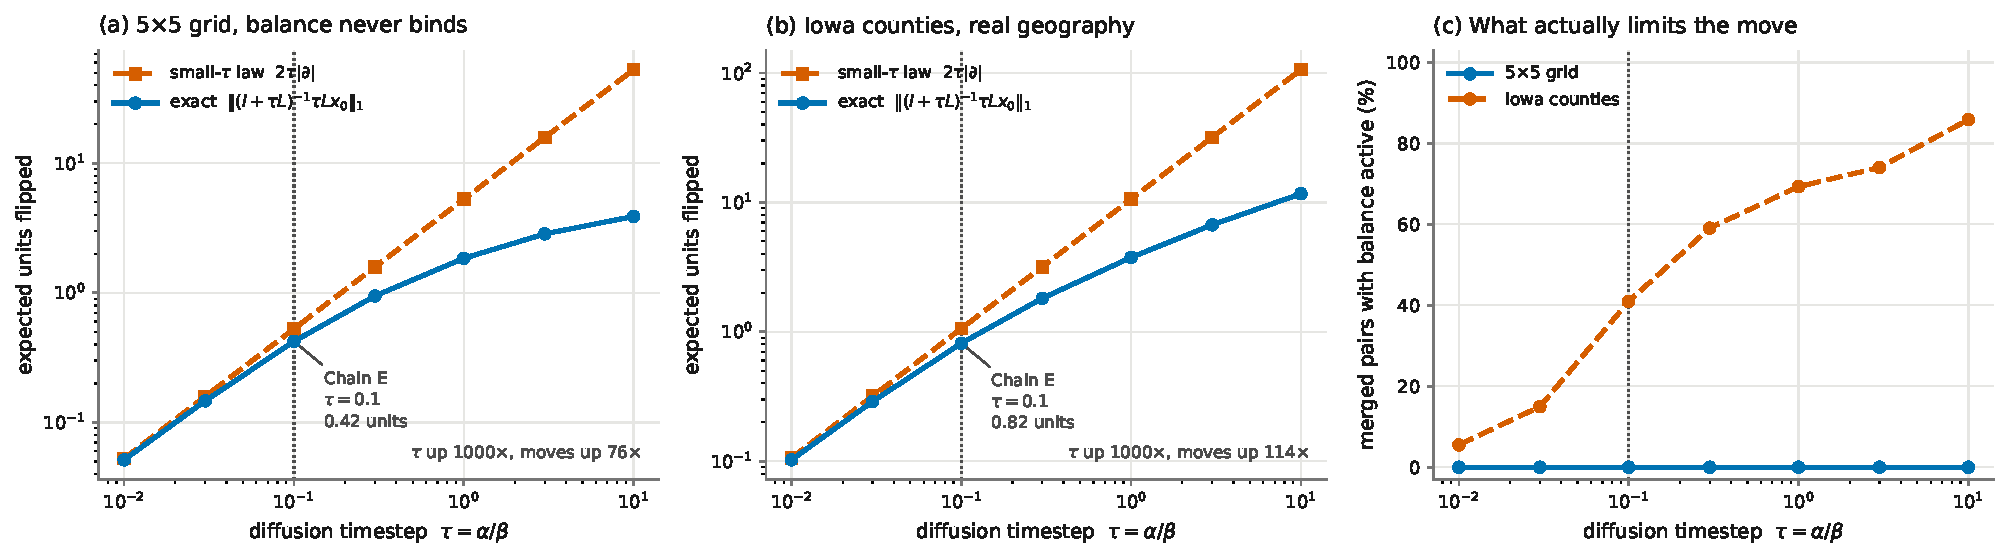
\includegraphics[width=\textwidth]{fig/spectral_move_size.pdf}
  \caption{The move-size law against the solver. (a)~On the enumerated
    $5 \times 5$ fiber, 1\,411 merged pairs drawn from 200 plans; the
    exact filter norm of \eqref{eq:move-size} and the small-timestep
    law $2\tau|\partial_w|$ agree for $\tau \le 0.03$ and separate as
    the gain saturates. Raising $\tau$ by $1000\times$ raises the move
    by $76\times$, and the last decade buys $2.1\times$. The locked
    Chain E setting $\tau = 0.1$ is marked. (b)~The same on Iowa, 127
    pairs from 25 tree-partition plans. (c)~Fraction of merged pairs
    whose balance constraint is active. On the uniform grid it never
    is, so the proposal is a linear solve at every step; on real county
    geography it is active for 41\% of pairs at $\tau = 0.1$ and 86\%
    at $\tau = 10$, so there the population constraint, not the
    diffusion, caps the move.}
  \label{fig:spectral-move-size}
\end{figure}

\textbf{Verification.} Across 10\,766 linear solves on the two test
beds the unconstrained optimum never left the unit cube, as
Lemma~\ref{lem:row-stochastic} requires. On 120 merged pairs with
balance slack, Gurobi's constrained solution and the linear solve
agree to $1.1 \times 10^{-4}$, the solver tolerance, so the
implementation matches the theory. The median relative error of the
small-timestep law against the exact filter norm is $2.5\%$ at
$\tau = 0.01$, $7.4\%$ at $0.03$, and $24\%$ at $0.1$
(Figure~\ref{fig:spectral-move-size}). At the paper's locked Chain E
setting the expected move is $0.42$ units on the $5 \times 5$ fiber
and, on Iowa, $0.82$ on the pairs whose window stays slack at every
timestep and $1.26$ averaged over all 127 pairs, about one unit per
proposal, which is the quantitative content of the chain's stickiness
reported in \S\ref{sec:exp-5x5}.

\subsection{Deterministic rounding, and why it blocks the correction}\label{sec:rounding}

The continuous optimum $x^\star \in [0,1]^{|V_H|}$ must be rounded to
a bipartition. The natural deterministic choice is a Cheeger
sweep~\cite{chung1997spectral}, which sorts the entries of $x^\star$,
scans the thresholds, keeps the balanced and connected candidate with
the smallest cut, and repairs near-misses by flipping orphaned
components to the other side. As a proposal it has a defect no repair
fixes. An argmin-plus-sweep map is deterministic, so the reverse
proposal has zero probability and the Hastings ratio degenerates; a
chain built on it is a heuristic with no stationarity claim beyond
ergodicity. \S\ref{sec:qp-mh} replaces the sweep with single-shot
randomized rounding, which restores an everywhere-positive proposal
density and an exact correction. The same defect, in a different
guise, is why the forest move of \S\ref{sec:forest} must keep the
tree draw and the cut-edge draw random rather than optimized.

\subsection{The exactly reversible QP-MH chain (Chain E)}\label{sec:qp-mh}

Replacing the deterministic rounding of \S\ref{sec:rounding} with
\emph{single-shot randomized rounding} restores a tractable,
everywhere-positive proposal density and yields an exactly reversible
chain. One step of Chain E is as follows.

\begin{enumerate}
  \item Pick an adjacent district pair $(V_i, V_j)$ uniformly at random
    from the $|\mathrm{bp}(P)|$ boundary pairs of the current plan $P$;
  \item Solve the (deterministic) QP of Definition~\ref{def:qp} on
    $H$ for $x^\star \in [0,1]^{|V_H|}$;
  \item Draw the proposal $x' \in \{0,1\}^{|V_H|}$ by independent
    Bernoulli rounding from the \emph{clipped} optimum,
    $x'_v \sim \mathrm{Bern}\bigl(\mathrm{clip}(x^\star_v;
    \delta, 1-\delta)\bigr)$ with $\delta = 10^{-12}$,
    \emph{once}, with no retry on infeasibility. Clipping is part of the
    proposal's definition. The QP optimum can have active box bounds
    (coordinates exactly $0$ or $1$, e.g.\ at interior vertices pinned
    by the fidelity term), and sampling from the same clipped vector
    whose density enters the acceptance ratio is what makes the
    proposal law and its stated density identical, with every binary
    $x'$ receiving positive probability;
  \item Accept with probability
    \begin{equation}\label{eq:qpmh-accept}
      \min\Bigl(1,\;
      \frac{\pi(P')}{\pi(P)}\,
      \frac{q(x_0 \mid P', \{i,j\})}{q(x' \mid P, \{i,j\})}\,
      \frac{|\mathrm{bp}(P)|}{|\mathrm{bp}(P')|}\Bigr),
    \end{equation}
    where $q(\cdot \mid P, \{i,j\})$ is the Bernoulli product density
    induced by the QP optimum at the corresponding state, and proposals
    that violate contiguity or the balance
    window~\eqref{eq:balance-window} are rejected outright.
\end{enumerate}

Here $\pi$ is any target on plans; the paper uses
$\pi_w(P) \propto \exp(-\lambda\, w(\partial P))$ for a kernel $w$,
which reduces to the tempered cut-count target for the uniform
kernel, and in \S\ref{sec:hybrid} also the tree-weighted variant.

\begin{proposition}[Detailed balance of Chain E]\label{prop:qpmh-db}
Chain E satisfies detailed balance with respect to any target $\pi$ on
$\mathcal{P}_k(G; \varepsilon)$ that is positive on valid plans.
\end{proposition}

Throughout, fix the deterministic edge kernel $w$ (weight jitter is
never used in this chain) and write $\Omega = \mathcal{P}_k(G;
\varepsilon)$ for the space of valid plans. Plans are \emph{labeled}
assignments in this subsection, so that a Bernoulli draw and its
complement are distinct states and the proposal map is a bijection;
on unlabeled partitions the map is two-to-one and the transition
probability would need both terms. Since $\pi$ depends only on the
partition it is label-invariant, and forgetting labels after
sampling recovers the unlabeled law. For a plan $P$ and an adjacent
pair $\{i,j\} \in \mathrm{bp}(P)$ write $H = V_i \cup V_j$ and let
$x_0(P) \in \{0,1\}^{V_H}$ denote the indicator of $V_i$ on $H$ (the
pair is drawn from a sorted list, so which district plays the role of
$i$ is a deterministic function of the unordered pair). Say that
$P' \in \Omega$ is \emph{pair-adjacent} to $P \in \Omega$ if
$P' \ne P$, the two plans differ on exactly two districts $\{i,j\}$,
and $H = V_i \cup V_j$ is connected. This relation is clearly
symmetric in $P$ and $P'$.

\begin{lemma}[Proposal regularity]\label{lem:qpmh-regular}
Let $P, P' \in \Omega$ be pair-adjacent via districts $\{i,j\}$, and
suppose $\beta > 0$. Then:
\begin{enumerate}
  \item[(i)] $\{i,j\}$ is the unique unordered pair whose selection
    can generate the move $P \to P'$ or the move $P' \to P$, and it
    is selectable from both endpoints:
    $\{i,j\} \in \mathrm{bp}(P) \cap \mathrm{bp}(P')$.
  \item[(ii)] The QP of Definition~\ref{def:qp} on $H$ with the
    global window~\eqref{eq:balance-window} has the same (nonempty)
    feasible set for the forward and reverse solves, and its optimum
    is unique, hence a deterministic function of
    $(\text{endpoint}, \{i,j\})$.
  \item[(iii)] The clipped-Bernoulli density
    $q(\cdot \mid \cdot, \{i,j\})$ is bounded below by
    $\delta^{|V_H|} > 0$ on every binary labeling of $V_H$; in
    particular $q(x_0(P') \mid P, \{i,j\}) > 0$ and
    $q(x_0(P) \mid P', \{i,j\}) > 0$.
\end{enumerate}
\end{lemma}

\begin{proof}
(i) A step that selects pair $\{a,b\}$ relabels vertices only
between districts $a$ and $b$ and changes no other district. If
$P' \ne P$, at least one vertex of $H$ switched between $i$ and $j$,
so districts $i$ and $j$ both changed; any generating pair must
therefore equal $\{i,j\}$. For selectability, note that
$(V_i, V_j)$ and $(V_i', V_j')$ are both bipartitions of the
connected graph $H$ into nonempty parts (all four sets are nonempty
districts of valid plans), and every such bipartition is crossed by
at least one edge of $H$; hence the two districts are adjacent in
both plans.

(ii) The feasible set is $\{x \in [0,1]^{V_H} : \ell \le p^\top x
\le u\}$ with $\ell, u$ given by~\eqref{eq:balance-window}. It
depends only on $(H, \varepsilon, \bar{p})$, not on the endpoint, so
the forward and reverse solves optimize over the same set. It is
nonempty at both endpoints because the window
of~\eqref{eq:balance-window} is precisely the condition that both
sides of the split be valid districts, which $x_0(P)$ and $x_0(P')$
satisfy by validity of $P$ and $P'$. This is where globality is
essential. Anchoring the window to the merged-pair half
$(1 \pm \varepsilon)\,p(V_H)/2$ instead lets a valid plan fail its
own pair's window, zeroing a reverse density whose forward
counterpart is positive and destroying reversibility outright. The
objective $\alpha\, x^\top L_H x + \beta\, \|x - x_0\|^2$ has Hessian
$2(\alpha L_H + \beta I) \succ 0$ for $\beta > 0$, so the minimizer
over the (convex, compact, nonempty) feasible set exists and is
unique, and it is a function of $(L_H, x_0, \ell, u)$ only. Since
the kernel $w$ is deterministic, $L_H$ depends only on $H$, and
$x_0$ only on the endpoint and the pair.

(iii) Clipping maps the optimum into $[\delta, 1-\delta]^{V_H}$, so
every Bernoulli factor of the product density lies in
$[\delta, 1-\delta]$ and every outcome in $\{0,1\}^{V_H}$ has
probability at least $\delta^{|V_H|}$.
\end{proof}

\begin{proof}[Proof of Proposition~\ref{prop:qpmh-db}]
Let $K$ denote the transition kernel of Chain E and fix distinct
$P, P' \in \Omega$. If $P$ and $P'$ are not pair-adjacent, no single
step can produce either move. A step changes at most the two selected
districts, so a generating pair would have to be the differing pair;
if the plans differ on more than two districts no pair qualifies, and
if the union $H$ of the two differing districts is disconnected, that
pair is not adjacent in either plan and is never selected. Hence
$K(P, P') = K(P', P) = 0$ and detailed balance holds trivially.

Otherwise let $\{i,j\}$ be the unique generating pair, abbreviate
$q_{\to} = q(x_0(P') \mid P, \{i,j\})$ and
$q_{\gets} = q(x_0(P) \mid P', \{i,j\})$, and note that both are
positive and finite by Lemma~\ref{lem:qpmh-regular}(ii)--(iii).
Because the rounding is single-shot, $q_{\to}$ is the exact
probability that the proposal from $P$ with pair $\{i,j\}$ equals
$P'$. No renormalization by a feasibility event is involved (a
retry-until-feasible loop would replace $q$ by a conditional law
whose state-dependent normalizing constant does not cancel in the
ratio), and clipping \emph{before} sampling makes the sampled law and
the density in~\eqref{eq:qpmh-accept} the same object. Hence
\[
  K(P, P') \;=\; \frac{1}{|\mathrm{bp}(P)|}\; q_{\to}\;
  \alpha(P, P'), \qquad
  \alpha(P, P') = \min\Bigl(1,\;
  \frac{\pi(P')}{\pi(P)}\,
  \frac{q_{\gets}}{q_{\to}}\,
  \frac{|\mathrm{bp}(P)|}{|\mathrm{bp}(P')|}\Bigr).
\]
Multiplying through,
\[
  \pi(P)\, K(P, P') \;=\;
  \min\Bigl(
  \frac{\pi(P)\, q_{\to}}{|\mathrm{bp}(P)|},\;
  \frac{\pi(P')\, q_{\gets}}{|\mathrm{bp}(P')|}
  \Bigr),
\]
an expression symmetric under exchanging $(P, q_{\to})$ with
$(P', q_{\gets})$. The identical computation started from $P'$ gives
the same right-hand side, so
$\pi(P) K(P, P') = \pi(P') K(P', P)$.

It remains to check that the rejection pathways do not disturb this
identity. A Bernoulli draw whose split leaves a side empty,
disconnected, or outside the window~\eqref{eq:balance-window} is a
proposal onto a state of zero target mass and is rejected with
probability one, contributing only to the diagonal $K(P, P)$, for
which detailed balance is vacuous; the same applies to in-space
proposals rejected by~\eqref{eq:qpmh-accept}. Rejection on solver
failure is symmetric because, by
Lemma~\ref{lem:qpmh-regular}(ii), the solve is a deterministic
function of $(H, \{i,j\}, \text{endpoint})$, so a failure that
suppresses the move $P \to P'$ suppresses the reverse move
identically. Detailed balance of $K$ with respect to $\pi$ on
$\Omega$ follows, and with it stationarity of
$\pi$~\cite{tierney1998note}.
\end{proof}

\begin{remark}[Scope, verification, and ergodicity]\label{rem:qpmh-scope}
The proof treats the QP solve as exact; in floating point the
minimizer is computed to solver tolerance, and determinism of the
implementation (fixed kernel, no jitter, sorted pair enumeration) is
what the argument actually uses. As an end-to-end check, we assembled
the full transition kernel of the implementation on an exhaustively
enumerated $2 \times 3$ grid ($k = 2$, tolerance $\varepsilon = 1/3$,
so that the 18 labeled valid states include $4{+}2$ as well as
$3{+}3$ splits) and verified
$\pi(P)K(P,P') = \pi(P')K(P',P)$ entrywise, with maximum relative
violation $1.5 \times 10^{-15}$ (machine precision;
\texttt{db\_check\_2x3.py}). Detailed balance
gives stationarity, not ergodicity. Within a selected pair every
binary relabeling of $H$ has positive proposal probability by
Lemma~\ref{lem:qpmh-regular}(iii), but irreducibility of Chain E
across pairs on general $(G, k, \varepsilon)$ is not established, so
convergence statements are for the chain restricted to its
communicating class. On the enumerated $5 \times 5$ fiber the chain's
cut distribution is indistinguishable from its target
(\S\ref{sec:exp-longrun}), on the $2 \times 3$ fiber a million-step
run's full occupancy distribution is (\S\ref{sec:exp-2x3}), and the
principled route to global mobility is the mixture of
\S\ref{sec:hybrid}.
\end{remark}

Chain E trades mobility for exactness. Because a proposal must be
feasible in a single Bernoulli draw, and because
Corollary~\ref{cor:small-tau} caps how far a draw can reach, the
chain behaves as a strictly local sampler. \S\ref{sec:mobility}
measures exactly why, and the answer is feasibility rather than the
Metropolis ratio. We therefore present Chain E as the local component
of the sampler rather than as a practical standalone sampler. Mixing
E with a global kernel preserves $\pi$ only if that kernel is
\emph{also} $\pi$-invariant. RevReCom as published is reversible with
respect to its spanning-tree measure, not an arbitrary $\pi$, so a
naive mixture would preserve neither; the correct construction
Metropolizes the tree move toward $\pi$ using its computable Hastings
ratio~\cite{cannon2022spanning,autry2023metropolized} and mixes
\emph{that} kernel with E, which is the construction of
\S\ref{sec:hybrid}.

\paragraph{On the tempered baseline (Chain A).} Our Tempered ReCom
baseline applies the filter $\min(1, \exp(-\lambda \Delta|\partial P|))$
over the ReCom proposal, which \emph{assumes a symmetric proposal}.
ReCom's proposal is not symmetric; the true Hastings ratio involves
spanning-tree counts of the affected
districts~\cite{autry2023metropolized,cannon2022spanning}, so Chain A
targets $\pi$ only approximately, and \S\ref{sec:exp-longrun}
quantifies the bias on enumerated ground truth. We keep the
symmetric-$q$ baseline because it is what practitioners run.

\subsection{Mobility of the exact chain: feasibility, not acceptance}\label{sec:mobility}

Proposition~\ref{prop:move-size} says how far a proposal reaches.
Mobility is that reach times the probability the proposal is kept,
and the second factor has two causes of different kinds. A Bernoulli
draw can produce a split that is disconnected or outside the balance
window, in which case it is rejected with probability one before any
coin is flipped. Or it can be a valid plan that loses the Metropolis
coin. We measured both on the enumerated $5 \times 5$ fiber, with
$\alpha = \tau$ and $\beta = 1$, over 3\,000 steps per timestep from
the same initial plan (Table~\ref{tab:mobility}).

\begin{table}[htbp]
\centering
\small
\begin{tabular}{rrrrrrrr}
\toprule
$\tau$ & $\E[\#\mathrm{flips}]$ & single-flip share & feasible $\mid$ single
  & $\Pr[\text{feasible}]$ & accept $\mid$ feasible & units moved / step & states \\
\midrule
0.01 & 0.036 & 0.035 & 0.000 & 0.964 & 1.000 & 0.0000 & 1 \\
0.03 & 0.126 & 0.110 & 0.000 & 0.884 & 1.000 & 0.0033 & 6 \\
0.10 & 0.385 & 0.268 & 0.000 & 0.683 & 0.999 & 0.0093 & 12 \\
0.30 & 0.909 & 0.349 & 0.000 & 0.437 & 0.989 & \textbf{0.0353} & \textbf{38} \\
1.00 & 1.914 & 0.254 & 0.000 & 0.193 & 0.983 & 0.0313 & 37 \\
3.00 & 2.672 & 0.168 & 0.000 & 0.074 & 0.986 & 0.0187 & 19 \\
\bottomrule
\end{tabular}
\caption{Chain E against the diffusion timestep on the $5 \times 5$
  fiber ($k = 5$, exact balance). ``Feasible $\mid$ single'' is the
  feasibility rate of single-unit proposals, ``accept $\mid$
  feasible'' the Metropolis acceptance rate among feasible
  proposals, and ``units moved / step'' the product of acceptance and
  accepted move size, the quantity a tuning rule should maximize.
  ``States'' counts distinct fiber states reached in 3\,000 steps.
  The locked setting of Appendix~\ref{app:hyperparams} is
  $\tau = 0.10$.}\label{tab:mobility}
\end{table}

Three facts follow. First, every single-unit proposal is infeasible at
every timestep, exactly as exact balance requires, since reassigning
one cell produces districts of sizes 4 and 6. The leading-order move
of the diffusion proposal is therefore always rejected on this fiber,
and the chain moves only through second-order coordinated draws. This
is the mechanism behind the coverage figures of \S\ref{sec:exp-5x5},
derived rather than observed. Second, the Metropolis ratio is never
the bottleneck. Given a feasible proposal, acceptance is between 98
and 100 percent throughout. The chain's stickiness is a feasibility
effect, and the natural phrase ``large moves are rarely accepted'' is
wrong in an instructive way. They are rarely feasible, and when
feasible they are accepted. Third, acceptance rate is a misleading
diagnostic for this chain. At $\tau = 0.01$ it is 96 percent while
the chain never leaves its initial state, because 96 percent of
proposals flip nothing. We report units moved per step instead.

Units moved per step has an interior maximum near $\tau = 0.3$. The
setting locked in Appendix~\ref{app:hyperparams}, $\tau = 0.1$, sits
about $3.8\times$ below it, so on this fiber the chain can be improved
for free; \S\ref{sec:exp-hybrid} shows the optimum does not transfer
to Iowa, where the balance window binds more often at larger $\tau$,
and \S\ref{sec:exp-scaling} shows that on large pairs the dial has to
be turned the other way. Even at the optimum a thousand steps move
about 35 units, and Corollary~\ref{cor:small-tau} says no timestep can
lift the per-proposal reach above half the merged pair. Both
statements matter. Chain E can be several times more mobile than
shown, and several times is not enough, which is why a global move is
required (\S\ref{sec:hybrid}). Under a loose tolerance single flips
become feasible and mobility gains a first-order term in $\tau$, which
is why the same chain climbs steadily on Iowa
(\S\ref{sec:exp-iowa-calib}) while freezing on the exact-balance grid.

\textbf{The mobility law.} On an exact-balance fiber the cheapest
feasible draw is a swap, one unit $u \in V_i$ and one unit $v \in V_j$
changing sides together, which preserves both populations. Rounding
flips units independently with probabilities
$p_v = |x^\star_v - x_{0,v}|$, so the probability that exactly
$\{u,v\}$ flips is $p_u p_v \prod_{w \ne u,v}(1 - p_w)$, and the
two-swap channel contributes
\begin{equation}\label{eq:mobility-law}
  M_2 \;=\; 2 \sum_{\substack{u \in V_i,\; v \in V_j \\ \text{swap feasible}}}
  p_u\, p_v \prod_{w \ne u,v} (1 - p_w)\;\alpha(u,v)
\end{equation}
units per step, where the sum runs over cross-boundary pairs whose
swap keeps both districts connected and $\alpha(u,v)$ is the
Metropolis probability of that swap, each of which costs one reverse
linear solve. For small $\tau$, $p_v = \tau b_v + O(\tau^2)$ with
$b_v$ the kernel weight of $v$'s cross-boundary edges, so
$M_2 = 2\tau^2 S_2 + O(\tau^3)$ with
$S_2 = \sum_{\text{feasible swaps}} b_u b_v$, a coefficient computable
from the current plan. We checked the law by running Chain E for
$20\,000$ steps per timestep and evaluating \eqref{eq:mobility-law}
at every step for the pair chosen and the plan visited
(Table~\ref{tab:mobility-law}).

\begin{table}[htbp]
\centering
\small
\begin{tabular}{rrrrr}
\toprule
$\tau$ & measured units / step & $M_2$ & $M_2$ without $\alpha$ & $2\tau^2 S_2$ \\
\midrule
0.03 & 0.0021 & 0.0018 & 0.0024 & 0.0033 \\
0.10 & 0.0105 & 0.0105 & 0.0127 & 0.0341 \\
0.30 & 0.0320 & 0.0326 & 0.0383 & 0.3628 \\
\bottomrule
\end{tabular}
\caption{The mobility law against Chain E on the $5 \times 5$ fiber,
  $20\,000$ steps per timestep. The two-swap channel with its
  Metropolis factor matches the measured mobility to within counting
  noise at every timestep; the $\tau = 0.03$ run holds 21 accepted
  swaps.}\label{tab:mobility-law}
\end{table}

The two-swap channel accounts for the chain's mobility at every
timestep tested, and four-unit draws contribute nothing measurable
even at $\tau = 0.3$. The Metropolis factor is not optional. Without
it the channel overpredicts by about $20\%$, because the chain's
near-unit acceptance given feasibility is dominated by zero-flip
proposals, and a genuine swap that lengthens the boundary is accepted
less often. The small-timestep form is accurate only for
$\tau \lesssim 0.03$, a narrower range than the move-size law's, as
expected for a second-order quantity. Under a loose tolerance single
flips become feasible, the law gains a first-order channel, and the
same calculation applies with single units in place of swaps.

\subsection{Exact tree moves, the lifted local move, and the reversible hybrid}\label{sec:hybrid}

Corollary~\ref{cor:small-tau} says the local chain cannot be made
mobile by tuning, so a global move is needed, and \S\ref{sec:qp-mh}
says that move must be reversible for the same target. This
subsection gives two exact tree moves, the one we use and the one
that explains Chain A, lifts Chain E to the state space of the first,
and states the sampler. It ends with the fact that organizes the
experiments: an exact tree move proposes from one fixed law, and pays
for every target that differs from it.

\subsubsection{The partition-level tree move (Chain T)}\label{sec:tree-partition}

Pick an adjacent pair $\{i,j\}$ uniformly from $\mathrm{bp}(P)$, draw
a uniform spanning tree $T$ of $H = G[V_i \cup V_j]$ by Wilson's
algorithm, and pick one edge of $T$ uniformly among \emph{all}
$|V_H| - 1$ tree edges. If the two components $A, B$ both lie in the
window~\eqref{eq:balance-window}, assign the labels $i, j$ to them by
a fair coin and propose; otherwise reject. Every spanning tree of $H$
that yields $\{A, B\}$ on removal of one edge is a spanning tree of
$G[A]$, a spanning tree of $G[B]$, and one crossing edge, so
\[
  q(P \to P') \;=\;
  \frac{\tau(A)\,\tau(B)\,|\partial(A,B)|}
       {2\,|\mathrm{bp}(P)|\,\tau(H)\,(|V_H| - 1)},
\]
where $\tau(\cdot)$ is the spanning-tree count by the Matrix--Tree
theorem and $|\partial(A,B)|$ the number of edges between $A$ and $B$.
The reverse move shares $H$, so $\tau(H)$ and $|V_H| - 1$ cancel and
the move is accepted with probability
\[
  \min\Bigl(1,\;
  \frac{\pi(P')}{\pi(P)}\;
  \frac{\tau(V_i)\,\tau(V_j)\,|\partial(V_i,V_j)|}
       {\tau(A)\,\tau(B)\,|\partial(A,B)|}\;
  \frac{|\mathrm{bp}(P)|}{|\mathrm{bp}(P')|}\Bigr),
\]
computable from four determinants and two edge counts. The fair coin
makes the move a bijection on labeled plans. The cut edge is drawn
among all tree edges rather than among balanced ones, and that is the
point of this move for us. GerryChain's \texttt{recom} draws among
balanced edges, which multiplies the density by a tree-dependent
normalization that does not cancel at the partition level, and that
is precisely why Chain A is only approximately correct. The price of
the closed form is acceptance. Most tree edges split a merged pair
unevenly, so the move accepts about $7\%$ of proposals on the
exact-balance $5 \times 5$ fiber and about $1\%$ on Iowa at
$\varepsilon = 0.05$. It is not what practice runs, and an earlier
version of this work used it as the baseline for the hybrid; the
numbers in \S\ref{sec:exp-hybrid} show why that was the wrong
comparison.

\subsubsection{The forest move (Chain F)}\label{sec:forest}

Recovering balanced-edge selection with an exact density means
lifting the state to a spanning forest, as Metropolized forest
recombination does~\cite{autry2023metropolized}. A labeled forest is
$\mathcal{F} = (P, \{T_d\})$, where $T_d$ is a spanning tree of
$G[V_d]$ for every district. The fiber over a plan $P$ has
$\tau(P) = \prod_d \tau(V_d)$ forests, and the lifted target
\begin{equation}\label{eq:lifted-target}
  \tilde\pi(\mathcal{F}) \;=\; \frac{\pi(P(\mathcal{F}))}{\tau(P(\mathcal{F}))}
\end{equation}
has marginal $\pi$ on plans. Every statistic we report is a function
of the plan, so traces are comparable with the partition-level
chains.

\textbf{One step.} Pick $\{i,j\}$ uniformly from $\mathrm{bp}(P)$ and
draw a uniform spanning tree $T$ of $H$. Let $B(T)$ be the set of
edges of $T$ whose removal leaves both components inside the
window~\eqref{eq:balance-window}. If $B(T)$ is empty, draw again, up
to $M$ times, then reject. Otherwise pick $e \in B(T)$ uniformly, let
$\{A, B\}$ be the components, and assign the labels by a fair coin. A
forest $\mathcal{F}' = (\ldots, T_A, T_B, \ldots)$ is reached from
exactly those draws $(\hat T, \hat e)$ with $\hat T = T_A \cup T_B \cup f$
for a crossing edge $f \in \partial(A,B)$ and $\hat e = f$, so
\begin{equation}\label{eq:forest-q}
  q(\mathcal{F} \to \mathcal{F}') \;=\;
  \frac{c_H}{2\,|\mathrm{bp}(P)|\,\tau(H)}\; S(T_A, T_B),
  \qquad
  S(T_A, T_B) \;=\; \sum_{f \in \partial(A,B)} \frac{1}{|B(T_A \cup T_B \cup f)|},
\end{equation}
where $c_H = (1 - (1 - p_H)^M)/p_H$ accounts for the retry, $p_H$
being the probability that a uniform spanning tree of $H$ has a
balanced edge. The retry is exact because $p_H$ depends on $H$ and
the window only, never on the endpoint, and the reverse move shares
$H$, so $c_H$ and $\tau(H)$ cancel. (This is not true of the local
move's rounding, whose feasibility event depends on the QP optimum at
the endpoint; that is why Chain E must be single-shot.) The Hastings
ratio is
\begin{equation}\label{eq:forest-ratio}
  \frac{\pi(P')}{\pi(P)}\;\cdot\;
  \frac{\tau(V_i)\,\tau(V_j)}{\tau(A)\,\tau(B)}\;\cdot\;
  \frac{S(T_i, T_j)}{S(T_A, T_B)}\;\cdot\;
  \frac{|\mathrm{bp}(P)|}{|\mathrm{bp}(P')|},
\end{equation}
where the tree-count ratio is the lifted target's, not the
proposal's. Each $S$ is a sum over the crossing edges of an $O(n)$
subtree-population pass, and the two determinants of the current
districts are cached, so a step costs two determinants plus
$O(|\partial|\, n)$. Our implementation differs from Autry et al.\ in
one convention: the adjacent pair is drawn uniformly from boundary
pairs, as in every other move of this paper, rather than by a uniform
cut edge; both are exact and the ratio carries the corresponding
factor.

\textbf{Two targets.} Besides $\pi_w(P) \propto e^{-\lambda\, w(\partial P)}$
we also use its tree-weighted version
$\pi_w^{\mathrm{tree}}(P) \propto \tau(P)\, e^{-\lambda\, w(\partial P)}$,
the measure that \S\ref{sec:exp-5x5} identifies as close to what
tempered ReCom samples. Under $\pi_w^{\mathrm{tree}}$ the tree-count
ratio in \eqref{eq:forest-ratio} cancels against the same factor in
$\pi(P')/\pi(P)$. Both targets are handled by the same code path; the
local move's acceptance under the tree-weighted target acquires the
tree-count ratio instead, since it changes the plan and hence
$\tau(P)$.

\subsubsection{The lifted local move and the hybrid (Chain H)}\label{sec:lifted-local}

Run Chain E on the plan against the chosen target. If it accepts,
redraw the trees of the two changed districts uniformly by Wilson's
algorithm; otherwise keep the forest. With $K_E$ $\pi$-reversible on
plans, the lifted kernel is
$\tilde K(\mathcal{F}, \mathcal{F}') = K_E(P, P') / (\tau(A)\tau(B))$,
and $\tilde\pi(\mathcal{F})\tilde K(\mathcal{F}, \mathcal{F}')$ is
symmetric because $\tau(P) = \tau(V_i)\tau(V_j)$ times the other
districts' counts, which the move does not change. Where the balance
window is slack the local solve is the linear solve of
Lemma~\ref{lem:row-stochastic}, which we use in place of the QP
solver; both paths are deterministic functions of the state and pair,
which is all Proposition~\ref{prop:qpmh-db} requires.

The hybrid takes a lifted local step with probability
$p_{\mathrm{loc}}$ and a forest step otherwise. Both kernels are
$\tilde\pi$-reversible, so the mixture is, and its marginal on plans
is $\pi$.

\begin{proposition}[Ergodicity of the hybrid]\label{prop:ergodic}
If the forest move is irreducible on the lifted space (which holds
under the standard assumptions for recombination moves;
see~\cite{deford2021recombination,cannon2024irreducibility,autry2023metropolized}),
then the mixture with the lifted local move at any
$p_{\mathrm{loc}} \in (0, 1)$ is ergodic.
\end{proposition}

\begin{proof}
Write $K = (1 - p_{\mathrm{loc}}) K_{\mathrm{F}} + p_{\mathrm{loc}}
\tilde K_{\mathrm{E}}$. If $K_{\mathrm{F}}^{t}(\mathcal{F}, \mathcal{F}') > 0$
for some $t$, then
$K^{t}(\mathcal{F}, \mathcal{F}') \ge (1 - p_{\mathrm{loc}})^{t}\,
K_{\mathrm{F}}^{t}(\mathcal{F}, \mathcal{F}') > 0$, so irreducibility
of the forest move implies irreducibility of the mixture. The forest
move rejects with positive probability at every state, so
$K(\mathcal{F}, \mathcal{F}) > 0$ and the chain is aperiodic.
\end{proof}

\textbf{Verification.} On the lifted $2 \times 3$ fiber (18 labeled
plans, 30 forests) we assembled the forest kernel, the lifted local
kernel with the linear-solve path, and their mixture analytically and
checked $\tilde\pi(\mathcal{F})K(\mathcal{F},\mathcal{F}') =
\tilde\pi(\mathcal{F}')K(\mathcal{F}',\mathcal{F})$ entrywise. The
maximum relative violation is $2.4 \times 10^{-16}$ for the forest
move, $1.4 \times 10^{-15}$ for the lifted local move, and
$2.6 \times 10^{-16}$ for the mixture under the uniform kernel at
$\lambda = 0.1$, and $4.1 \times 10^{-16}$, $1.1 \times 10^{-15}$ and
$6.0 \times 10^{-16}$ under a density kernel at $\lambda = 1$, for
both targets. The closed-form proposal mass
\eqref{eq:forest-q} equals the mass obtained by enumerating every
(tree, balanced edge, coin) draw to $1.8 \times 10^{-16}$
(\texttt{forest\_recom.py}). The same check for the partition-level
chains T, E and their mixture gives $4.8 \times 10^{-16}$,
$1.6 \times 10^{-15}$ and $7.2 \times 10^{-16}$ (\texttt{hybrid.py}).
\S\ref{sec:exp-hybrid} tests the forest move and the hybrid against
enumerated targets on 4\,006 plans.

\subsubsection{What an exact tree move pays}\label{sec:tree-pays}

Both tree moves draw the proposed split from the same law, the
spanning-tree measure on balanced bipartitions of $H$ conditioned on
nothing else: Chain T from it exactly, Chain F from it up to the
$S$ factor, which the experiments below show to be within a factor of
two of one. Given the pair, the proposed split does not depend on the
current one. On a merged pair the tree move is therefore an
\emph{independence sampler}, and its acceptance at equilibrium is
governed by how far the target's conditional on the pair sits from
that law. Two terms of \eqref{eq:forest-ratio} carry the distance.
Under $\pi_w$ the tree-count ratio does: a uniform spanning tree
favors splits with many spanning trees, and by Procaccia and
Tucker-Foltz~\cite{procaccia2022compact} the logarithm of a tree
count scales with the boundary length, so at the equilibrium of a
target that is less compact than the tree measure the ratio is
typically far below one. Under $\pi_w^{\mathrm{tree}}$ that ratio
cancels and the target ratio $e^{-\lambda \Delta w(\partial)}$
carries the distance instead, which is large whenever the tempering
makes the target more compact than an untempered tree split.

We measured the terms on Iowa over 3\,000 forest proposals from a
tree-partition start under $\pi_w$ (Table~\ref{tab:decomposition}).
The tree-count term dominates, with mean logarithm $-6$ to $-10$ and
a share of $67$ to $84$ percent of feasible proposals below $e^{-2.3}$
on that term alone, while the target, $S$ and pair-count terms are
mild. At the equilibrium of the uniform target the acceptance given a
feasible tree is $0.17$; under the tree-weighted target at the same
temperature it is $0.74$, because at $\lambda$ equivalent to $0.1$
that target is close to the untempered tree measure. The scaling
experiment of \S\ref{sec:exp-scaling} then shows what happens as the
pair grows: for a compactness-tempered target, with or without tree
weights, the mismatch grows in proportion to the boundary length and
the acceptance decays exponentially in the grid side. The local move
loses acceptance with pair size as well, because its expected move
grows with the boundary (Corollary~\ref{cor:small-tau}), but it has a
dial for it, the timestep; the tree move has none, since its proposal
is the same law whatever the target.

\begin{table}[htbp]
\centering
\small
\begin{tabular}{lrrrrrrr}
\toprule
target & $\Pr[\text{tree balanced}]$ & accept $\mid$ feasible &
 \multicolumn{4}{c}{mean of each log term} & share with $\tau$-term $< e^{-2.3}$ \\
\cmidrule(lr){4-7}
 & & & target & tree count & $S$ & bp & \\
\midrule
uniform, $\lambda = 0.10$   & 0.41 & 0.25 & $+0.63$ & $-5.93$ & $+0.47$ & $-0.01$ & 0.67 \\
perimeter, $\lambda = 0.34$ & 0.53 & 0.22 & $+0.65$ & $-5.98$ & $+0.59$ & $-0.00$ & 0.69 \\
density, $\lambda = 0.72$   & 0.41 & 0.13 & $+1.62$ & $-9.78$ & $+0.74$ & $-0.06$ & 0.84 \\
\bottomrule
\end{tabular}
\caption{The four terms of the forest move's log Hastings
  ratio~\eqref{eq:forest-ratio} on Iowa ($k = 4$,
  $\varepsilon = 0.05$) under $\pi_w$, averaged over the feasible
  proposals of 3\,000 steps from a tree-partition start, without
  retry. The tree-count ratio is the rejection; the retry raises
  $\Pr[\text{tree balanced}]$ to $0.95$ at $2.5$ times the wall clock
  and leaves accepted moves per second unchanged.}\label{tab:decomposition}
\end{table}

%════════════════════════════════════════════════════════════════════════════════
\section{Experiments}\label{sec:experiments}
%════════════════════════════════════════════════════════════════════════════════

We evaluate the chains of Table~\ref{tab:chains} on the
$5 \times 5$ grid (full enumeration, ground-truth target), the
$2 \times 3$ grid (18 states, full convergence checkable), the Iowa
county dual graph (real geography, 99 counties, $k = 4$,
$\varepsilon = 0.05$), and $N \times N$ grids with $k = 2$ for the
scaling experiment. All hyperparameters are locked in
Appendix~\ref{app:hyperparams}; raw traces, per-step balance audits,
and configuration stamps are released in the project repository.

\paragraph{Statistical protocol.} Chains are autocorrelated, so we do
not report i.i.d.\ test statistics on raw traces. Effective sample
sizes (ESS) come from Geyer's initial-positive-sequence estimator of
the integrated autocorrelation time, computed by FFT, and are
appropriate for inference about cut means only; distributional tests
use batch means (\S\ref{sec:exp-2x3}), and distances to enumerated
targets are read against parametric-bootstrap noise floors at the
ESS (\S\ref{sec:exp-longrun}). When two chains are compared by
effective samples per second we also report effective samples per
step, which does not depend on the implementation, and we check that
the two chains sit at the same level, by quarter means and by the
difference of their post-burn means in standard errors from their
own ESS. Each chain runs on its own seeded RNG stream; the baseline
tables report seed 42, and the ten-seed means of Chains V and A
(seeds 42 through 51) are quoted where they enter the calibration.
Between-seed standard deviations of the baselines are about $0.4$
cuts on Iowa and $0.1$ to $0.2$ cuts on the $5 \times 5$ fiber, so
single-seed means are representative.

\paragraph{Balance audit.}\label{sec:exp-balance} Every run of the
baseline chains records, at every step, the maximum relative
deviation of any district population from the global ideal, and all
of them satisfy the $\varepsilon = 0.05$ bound at every step (Iowa
maxima 0.0498--0.0500 for the runs of \S\ref{sec:exp-iowa-calib});
the exact chains of \S\ref{sec:hybrid} enforce the window inside each
move by construction, rejecting any draw outside it. We flag this
because it is not automatic.
GerryChain's raw \texttt{recom} proposal validates only one side of
each tree cut, and an earlier version of our own local steps anchored
balance to the merged-pair half rather than the global ideal
(\S\ref{sec:qp-model}); either slip lets district populations drift
to $\sim$4$\times$ the nominal tolerance on Iowa before the audit
catches it. We recommend per-step balance auditing as standard
practice for any custom chain harness that bypasses GerryChain's
validator pipeline.

\subsection{Ground truth on the enumerated fiber: what the family samples}\label{sec:exp-5x5}

The $5 \times 5$ partition fiber (the set of all valid plans; $k = 5$, exact balance, 4\,006
partitions; Appendix~\ref{sec:fiber-corridors}) admits full enumeration, so
every distributional quantity is exactly computable. The chains run
with $\varepsilon = 0.05$, which on 25 unit-population cells admits
only districts of exactly five cells, so the state space the chains
traverse is precisely this enumerated fiber. Uniform-on-fiber is not the target of any chain here; the
total-variation column is a descriptive concentration measure only,
and with about 900 correlated draws over 4\,006 states even an
independent uniform sampler would show TV above $0.78$. The
informative comparisons are the cut means against the exact target
mean and the long runs of \S\ref{sec:exp-longrun}, where distances
are read against proper noise floors. Table~\ref{tab:5x5-headline}
gives the short-run picture.

\begin{table}[htbp]
\centering
\small
\begin{tabular}{lrrrr}
\toprule
Chain & Mean cuts & Std & Unique / 4006 & TV(emp, uniform) \\
\midrule
V: Vanilla ReCom     & 17.06 & 1.08 & 337 / 4006 (8.4\%) & 0.92 \\
A: Tempered ReCom    & 17.02 & 1.15 & 311 / 4006 (7.8\%) & 0.92 \\
E: QP-MH exact       & 16.27 & 0.44 & \phantom{00}6 / 4006 (0.1\%) & 1.00 \\
\bottomrule
\end{tabular}
\caption{$5 \times 5$ short-run comparison ($k = 5$, exact balance,
  1\,000 steps, burn-in 100, seed 42). The exact target mean is
  $\E_\pi[|\partial P|] = 18.56$ at $\lambda = 0.10$, and \emph{every}
  chain sits far below it at this horizon, including the exactly
  reversible Chain E, which at 1\,000 steps has visited only 6 states. Exactness of the kernel does not buy mixing speed.}\label{tab:5x5-headline}
\end{table}

\textbf{The origin of the gap.} The
gap between every chain's empirical mean and the target mean 18.56
quantifies the compactness bias \emph{shared} by the whole
ReCom-derived family, and on the enumerated fiber we can identify its
origin. Using the Matrix--Tree theorem we compute, for each of the
4\,006 partitions, the spanning-tree-count weight
$\prod_i \tau(V_i)$, the measure that the RevReCom analysis
identifies as the natural target of tree-based
recombination~\cite{cannon2022spanning,autry2023metropolized} and
whose relation to compactness Procaccia and
Tucker-Foltz~\cite{procaccia2022compact} proved. At the level of
means the match is close. The tree-weighted measure has
$\E[|\partial P|] = 16.88$ against Vanilla ReCom's ten-seed mean of
$16.95 \pm 0.11$, and the tree-weighted-and-tempered measure
$\prod_i \tau(V_i)\, e^{-\lambda|\partial P|}$ has
$\E[|\partial P|] = 16.78$ against Chain A's ten-seed mean of
$16.71 \pm 0.16$; both gaps are 0.07 cuts, within one between-seed
standard deviation, and the two quasi-targets sit 1.7 and 1.8 cuts
below the nominal tempered mean. A mean is a one-dimensional summary,
though, and many distributions share one. The long runs below compare
full distributions, which is where the claim is actually tested.

\paragraph{Long-run validation at the level of distributions.}\label{sec:exp-longrun}
We run Chain A for $2 \times 10^5$ steps and Chain E for $10^5$ steps
on the enumerated fiber (seed 42, 10\% burn-in) and compare each
chain's empirical distribution against three exactly computable
reference measures, the nominal target
$\pi \propto e^{-\lambda|\partial P|}$, the tree-weighted measure
$\prod_i \tau(V_i)$, and the tree-weighted-and-tempered measure. Two
design choices make the comparison informative. First, a raw
total-variation distance is uninterpretable on 4\,006 states, since
even an independent sampler shows large TV until the draw count
greatly exceeds the state count. So every distance is reported
against a parametric-bootstrap noise floor, the same distance
computed for independent draws from the reference measure at the
chain's effective sample size. A converged chain sits at its floor; a
chain converging elsewhere sits above it by many floor standard
deviations. Second, the headline statistic is the cut-count marginal
rather than the full state distribution. The fiber's cut counts take
five values, so with $1.8 \times 10^5$ retained draws the marginal is
estimated to three decimals and its floor is small, which removes the
coverage problem entirely. Table~\ref{tab:calibration-tv} and
Figure~\ref{fig:calibration} give the result.

\begin{table}[htbp]
\centering
\small
\begin{tabular}{llrrr}
\toprule
Chain & Reference measure & TV & Floor at ESS & $z$ \\
\midrule
A ($2\times10^5$ steps, ESS 12\,312) & nominal $\pi$ & 0.629 & 0.007 & $+220$ \\
 & tree-weighted & 0.065 & 0.006 & $+22$ \\
 & tree-weighted, tempered & 0.022 & 0.006 & $+6.7$ \\
\midrule
E ($10^5$ steps, ESS 28) & nominal $\pi$ & 0.079 & 0.141 & $-1.2$ \\
 & tree-weighted & 0.493 & 0.125 & $+6.9$ \\
 & tree-weighted, tempered & 0.532 & 0.125 & $+7.5$ \\
\bottomrule
\end{tabular}
\caption{Total variation between each chain's empirical cut-count
  marginal and three reference measures on the enumerated
  $5 \times 5$ fiber, with the parametric-bootstrap noise floor at the
  chain's effective sample size and the excess in floor standard
  deviations. Chain A is far from its nominal target and close to,
  though distinguishable from, the tree-weighted tempered measure.
  Chain E is indistinguishable from the nominal target it is proved
  reversible for and far from the tree measures.}\label{tab:calibration-tv}
\end{table}

\begin{figure}[htbp]
  \centering
  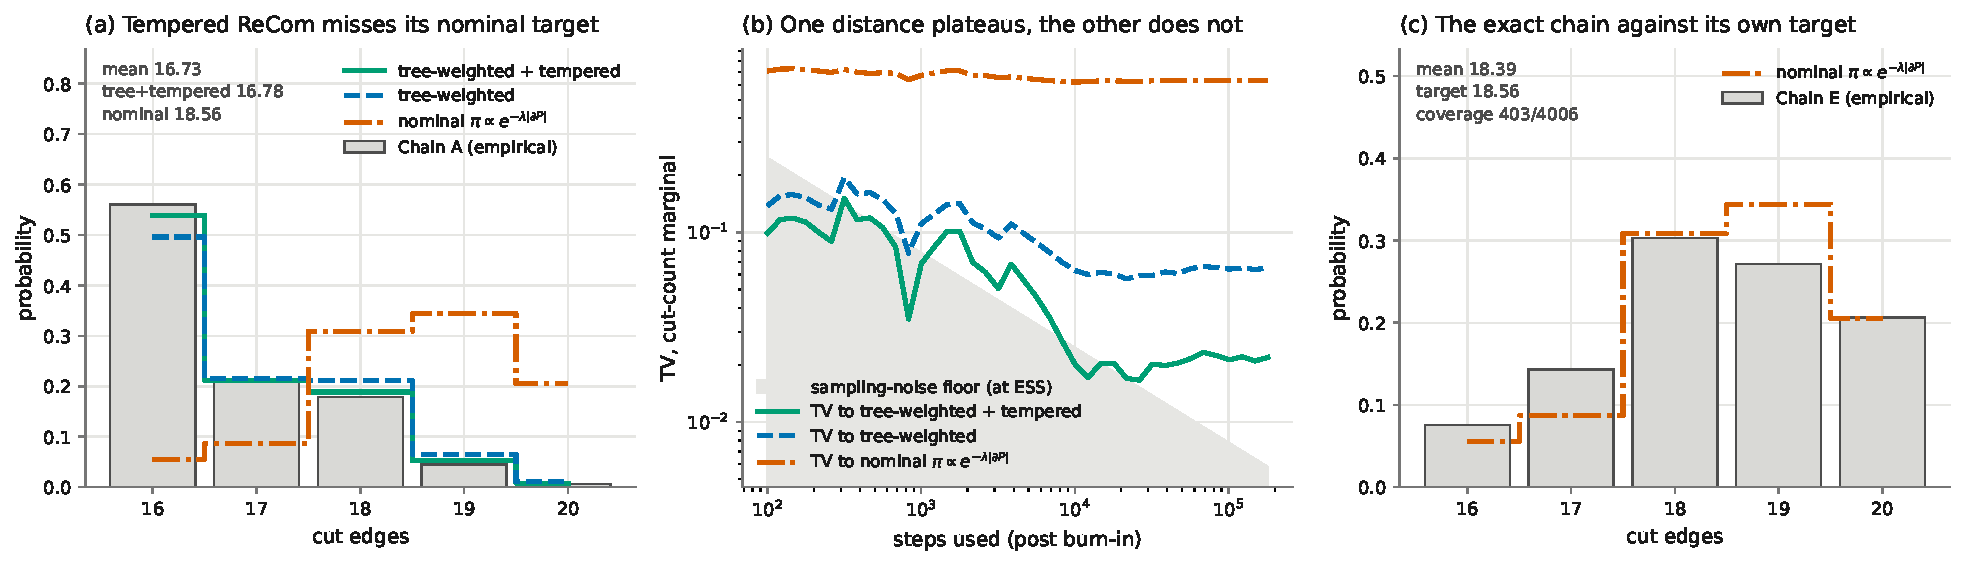
\includegraphics[width=\textwidth]{fig/calibration_5x5.pdf}
  \caption{What the chains sample. (a)~Chain A's cut-count marginal
    after $2 \times 10^5$ steps against the three reference measures.
    (b)~Total variation of the running marginal to each reference as a
    function of run length, with the noise floor at the effective
    sample size shaded; the distance to the nominal target is a
    plateau across five decades while the distance to the
    tree-weighted tempered measure descends toward the floor.
    (c)~Chain E's marginal after $10^5$ steps against its own
    target.}
  \label{fig:calibration}
\end{figure}

\emph{Chain A does not sample its nominal target, and the gap is a
plateau, not a drift.} At $2 \times 10^5$ steps the tempered chain
has visited $3\,524/4\,006$ states, its mean is $16.73$, and its cut
distribution sits 220 floor standard deviations from the nominal
target, at TV $0.63$. Figure~\ref{fig:calibration}(b) shows that
distance flat across five decades of run length while the distance
to the tree-weighted tempered measure falls toward the floor. This is
convergence to a different distribution, not slow mixing, and it is
what the symmetric-$q$ filter of \S\ref{sec:qp-mh} predicts. The
match to the tree-weighted tempered measure is close but not exact.
At TV $0.022$ the chain sits $6.7$ floor standard deviations above
it, so the tree measure is a very good description of what tempered
ReCom samples and not a perfect one, which is expected, since Vanilla
ReCom's stationary law is not exactly the tree measure and RevReCom
exists to make it so. On the full 4\,006-state distribution the noise
floor at effective sample size is $0.15$ to $0.23$, so that comparison
can separate the nominal target ($z = +164$) but not the two tree
measures from each other, which is why the marginal carries the
claim.

\emph{Chain E samples what it states.} At $10^5$ steps its cut
marginal is $1.2$ floor standard deviations from the nominal target
and about $7$ from either tree measure. The two chains separate
exactly as theory predicts. Convergence of the full distribution is
far slower for this sticky local chain, as \S\ref{sec:mobility}
explains. It has visited $403/4\,006$ states, and its full-state TV
of $0.90$ sits at a floor of $0.99$ at effective sample size 28, so
that test has no power here. The fiber on which full convergence can
be checked is the next subsection.

\subsection{Exact convergence on the 18-state fiber}\label{sec:exp-2x3}

Detailed balance gives stationarity, not convergence, and on 4\,006
states the exact chain cannot be run to convergence in reasonable
time. On the $2 \times 3$ grid with $k = 2$ and tolerance
$\varepsilon = 1/3$, the fiber of labeled valid plans has 18 states,
the same state space on which Remark~\ref{rem:qpmh-scope} verifies
the kernel to machine precision, and a long run can cover it. We run
Chain E for $10^6$ steps (seed 42, $10\%$ burn-in, locked parameters
$\alpha = 1$, $\beta = 10$, $\lambda = 0.10$). It visits all 18
states, its acceptance rate is $0.785$, and its post-burn-in mean cut
count is $2.75992$ against the exact $2.76002$.

The distributional test uses batch means, because thinning a chain by
an effective sample size computed from a summary statistic is not
valid here. The cut count takes two values on this fiber, so its
integrated autocorrelation time ($17$ steps) understates that of the
18-state occupancy process ($25$ steps), and a chi-square test on a
chain thinned by the former rejects spuriously. We therefore split
the trace into 200 blocks of $4\,500$ steps, over 180 occupancy
correlation times each, estimate the covariance of the occupancy
vector from the between-block scatter, and test with Hotelling's
$T^2$ on the 17 free coordinates. The result is $F(17, 183) = 0.87$,
$p = 0.61$. The occupancy distribution is not distinguishable from
the exact target. Total variation to the target is $0.0110$, against
a noise floor of about $0.009$ at the occupancy effective sample
size, and it fell from $0.0250$ at $2 \times 10^5$ steps, a factor of
$2.27$ for five times the steps, which is the $\sqrt{n}$ rate of a
converged chain. At $2 \times 10^5$ steps the same test gave
$p = 0.07$ with three states in one cut-level set persistently
under-visited; at $10^6$ steps those deviations dissolved into the
few $|z| \approx 2$ values that 18 states produce by chance.
Together with the kernel check, this is end-to-end validation of the
construction of \S\ref{sec:qp-mh}. The implemented kernel satisfies
detailed balance exactly, and the chain it generates reaches its
target.

\subsection{The forest move and the hybrid against enumerated targets}\label{sec:exp-hybrid}

We run the partition-level tree move (T), the forest move (F) and
the hybrid (H, $p_{\mathrm{loc}} = 0.2$, $\tau = 0.1$) from the same
start for $2 \times 10^5$ steps on the $5 \times 5$ fiber against
three enumerated targets, the uniform kernel at $\lambda = 0.1$ and
at $\lambda = 1$ and a density kernel at $\lambda = 1$ built from a
synthetic central city, $\rho(x,y) = 3\exp(-r^2/2)$ with
$w_{uv} = \exp(-(\rho_u - \rho_v)^2)$, under which $\pi_w$ favors
boundaries that follow the density gradient and the tree proposal is
blind to the kernel; and then the forest move and the hybrid against
the tree-weighted versions of the same three targets. Each chain is
tested as in \S\ref{sec:exp-longrun}, by the cut-count marginal
against its noise floor and by batch-means Hotelling (with cut bins
of negligible target mass merged, since under the sharp tree-weighted
target the top bin has mass $3 \times 10^{-4}$), and we report
effective samples per second. The pre-registered criterion for the
local move is the ratio of the hybrid's effective samples per second
to the forest move's: at or above $1.5$ the local move earns its
place, below $1$ it is a passenger.

\begin{table}[htbp]
\centering
\small
\begin{tabular}{llrrrrrrr}
\toprule
Target & Chain & TV marg & $z$ & Hotel.\ $p$ & acc global & acc local & ESS/s & ratio \\
\midrule
\multicolumn{9}{l}{\emph{target} $\pi_w$} \\
uniform, $\lambda{=}0.1$ & T & 0.010 & $-1.8$ & 0.58 & 0.066 & --- & 51.1 & \\
 & F & 0.006 & $-1.2$ & 0.46 & 0.851 & --- & 211.8 & F/T $4.15$ \\
 & H & 0.013 & $+0.2$ & 0.43 & 0.851 & 0.660 & 143.8 & H/F $0.68$ \\
uniform, $\lambda{=}1$ & T & 0.028 & $-0.8$ & 0.21 & 0.074 & --- & 45.2 & \\
 & F & 0.004 & $-1.3$ & 0.80 & 0.979 & --- & 338.6 & F/T $7.49$ \\
 & H & 0.005 & $-1.3$ & 0.83 & 0.979 & 0.673 & 240.3 & H/F $0.71$ \\
density, $\lambda{=}1$ & T & 0.028 & $-0.6$ & 0.60 & 0.069 & --- & 55.3 & \\
 & F & 0.004 & $-1.5$ & 0.96 & 0.876 & --- & 254.5 & F/T $4.61$ \\
 & H & 0.005 & $-1.5$ & 0.25 & 0.876 & 0.784 & 168.9 & H/F $0.66$ \\
\midrule
\multicolumn{9}{l}{\emph{target} $\pi_w^{\mathrm{tree}}$} \\
uniform, $\lambda{=}0.1$ & F & 0.009 & $+0.2$ & 0.37 & 0.944 & --- & 257.3 & \\
 & H & 0.006 & $-0.8$ & 0.78 & 0.942 & 0.675 & 188.8 & H/F $0.73$ \\
uniform, $\lambda{=}1$ & F & 0.003 & $-1.0$ & 0.64 & 0.884 & --- & 265.9 & \\
 & H & 0.005 & $-0.4$ & 0.41 & 0.886 & 0.683 & 182.3 & H/F $0.69$ \\
density, $\lambda{=}1$ & F & 0.007 & $+0.1$ & 0.46 & 0.906 & --- & 259.3 & \\
 & H & 0.003 & $-1.3$ & 0.70 & 0.906 & 0.789 & 168.6 & H/F $0.65$ \\
\bottomrule
\end{tabular}
\caption{Exact tree moves and the hybrid on the enumerated
  $5 \times 5$ fiber, $2 \times 10^5$ steps each, seed 42. ``TV
  marg'' is total variation of the cut-count marginal to the
  enumerated target and $z$ its excess over the noise floor at the
  effective sample size; ``Hotel.\ $p$'' is the batch-means test of
  \S\ref{sec:exp-2x3}; ESS is of the weighted-cut trace, timed in the
  same session.}\label{tab:hybrid-5x5}
\end{table}

Three findings. First, every chain samples its target. All fifteen
rows sit within $1.8$ floor standard deviations of the enumerated
marginal with Hotelling $p$ between $0.21$ and $0.96$, under both
target families and both kernels, so the forest move, the lifted
local move and their mixture are correct for kernel-weighted targets
on 4\,006 states and not only on the 30 lifted states of the analytic
check. Second, the forest move is a different baseline from the
partition-level tree move: it accepts $0.85$ to $0.98$ against $0.07$,
and delivers $4$ to $7.5$ times the effective samples per second on
this fiber. Third, on this fiber the local move is a passenger under
every target, with ratios $0.65$ to $0.73$. That is what
\S\ref{sec:mobility} predicts under exact balance, where the local
move's first-order channel is closed, and it is also what
\S\ref{sec:tree-pays} predicts for pairs of ten cells, where the
mismatch between any of these targets and the tree measure is small.
The grid tells us the construction is right and tells us nothing yet
about where the local move matters; Iowa and the scaling experiment
do.

\subsection{The kill test on Iowa}\label{sec:exp-iowa}

On Iowa ($k = 4$, $\varepsilon = 0.05$) there is no ground truth, so
the comparison is mobility at equilibrium. We use the paper's three
kernels with $\lambda$ scaled so that $\lambda\, w(\partial P)$ at the
initial plan equals the uniform case's $0.1\,|\partial P|$, and run
the forest move alone and the hybrid at $p_{\mathrm{loc}} \in \{0.1,
0.3\}$, $\tau = 0.1$. The criterion was fixed before the long runs
were started: under $\pi_w$, with $p_{\mathrm{loc}} = 0.1$, the hybrid
passes if its effective samples per second are at least $1.5$ times
the forest move's on both the perimeter and the density target on
both seeds, with the two chains at the same level. The
$p_{\mathrm{loc}} = 0.3$ runs were added after the short runs favored
that setting and are reported as a secondary finding.

\paragraph{Short runs, direction and timing.} Table~\ref{tab:iowa-short}
gives $2 \times 10^5$ steps per chain. Under $\pi_w$ the forest move
accepts $0.16$ to $0.17$, the partition-level tree move $0.006$ to
$0.012$, and yet the two deliver similar effective samples per second,
because a forest step costs six times more (every feasible draw pays
the determinants and the crossing-edge sums) and the partition-level
move pays them only on the one percent of draws that balance. The
hybrid beats the forest move on every kernel, by $1.4$ to $1.8$ at
$p_{\mathrm{loc}} = 0.1$ and $2.4$ to $4.4$ at $0.3$, but the forest
move's effective sample size in these runs is $36$ to $56$, so these
ratios carry roughly $40$ percent uncertainty. Under
$\pi_w^{\mathrm{tree}}$ the picture inverts: the forest move accepts
$0.66$ to $0.74$, its effective sample size is about $10\,000$ per
$2 \times 10^5$ steps, two hundred times its value under $\pi_w$ at
the same step count, and the hybrid is a passenger at $0.86$ to
$0.93$.

\begin{table}[htbp]
\centering
\small
\begin{tabular}{llrrrrrrr}
\toprule
Target & Chain & acc global & acc local & $\bar w$ 1st half & $\bar w$ 2nd half & ESS & ESS/s & ratio \\
\midrule
\multicolumn{9}{l}{$\pi_w$} \\
uniform, $\lambda{=}0.10$ & F & 0.163 & --- & 89.2 & 87.8 & 36 & 0.161 & --- \\
 & H, $p{=}0.1$ & 0.158 & 0.249 & 90.1 & 89.4 & 56 & 0.223 & 1.39 \\
 & H, $p{=}0.3$ & 0.165 & 0.254 & 89.8 & 89.3 & 180 & 0.714 & 4.44 \\
 & T & 0.012 & --- & 83.2 & 87.2 & 14 & 0.395 & 2.46 \\
perimeter, $\lambda{=}0.34$ & F & 0.163 & --- & 28.1 & 28.2 & 43 & 0.185 & --- \\
 & H, $p{=}0.1$ & 0.163 & 0.530 & 28.7 & 28.2 & 79 & 0.339 & 1.83 \\
 & H, $p{=}0.3$ & 0.158 & 0.526 & 28.0 & 28.4 & 116 & 0.450 & 2.44 \\
 & T & 0.006 & --- & 25.5 & 28.2 & 6 & 0.153 & 0.83 \\
density, $\lambda{=}0.72$ & F & 0.174 & --- & 18.3 & 17.9 & 56 & 0.243 & --- \\
 & H, $p{=}0.1$ & 0.173 & 0.672 & 18.1 & 18.1 & 93 & 0.424 & 1.74 \\
 & H, $p{=}0.3$ & 0.174 & 0.669 & 18.2 & 18.1 & 174 & 0.852 & 3.51 \\
 & T & 0.007 & --- & 13.3 & 14.8 & 6 & 0.204 & 0.84 \\
\midrule
\multicolumn{9}{l}{$\pi_w^{\mathrm{tree}}$} \\
uniform, $\lambda{=}0.10$ & F & 0.741 & --- & 41.05 & 40.93 & 10\,035 & 60.6 & --- \\
 & H, $p{=}0.1$ & 0.742 & 0.419 & 40.98 & 40.94 & 10\,677 & 56.4 & 0.93 \\
 & H, $p{=}0.3$ & 0.744 & 0.422 & 41.05 & 40.90 & 8\,010 & 34.2 & 0.56 \\
perimeter, $\lambda{=}0.34$ & F & 0.733 & --- & 13.04 & 13.04 & 10\,257 & 62.3 & --- \\
 & H, $p{=}0.1$ & 0.732 & 0.714 & 13.04 & 13.03 & 9\,459 & 54.2 & 0.87 \\
 & H, $p{=}0.3$ & 0.735 & 0.715 & 13.06 & 13.04 & 7\,686 & 40.2 & 0.64 \\
density, $\lambda{=}0.72$ & F & 0.662 & --- & 7.30 & 7.31 & 9\,295 & 53.7 & --- \\
 & H, $p{=}0.1$ & 0.662 & 0.831 & 7.34 & 7.27 & 8\,334 & 46.0 & 0.86 \\
 & H, $p{=}0.3$ & 0.660 & 0.832 & 7.28 & 7.29 & 5\,927 & 34.7 & 0.65 \\
\bottomrule
\end{tabular}
\caption{Iowa short runs ($k = 4$, $\varepsilon = 0.05$,
  $2 \times 10^5$ steps, seed 42, $\tau = 0.1$). The two $\bar w$
  columns are the mean weighted cut over the halves of the retained
  trace; ``ratio'' is effective samples per second relative to the
  forest move at the same target, timed in the same session. The
  partition-level tree move T is included under $\pi_w$ for the
  baseline-against-baseline comparison; it has no tree-weighted
  implementation.}\label{tab:iowa-short}
\end{table}

\paragraph{Long runs, the verdict.} Table~\ref{tab:iowa-long} gives
$2 \times 10^6$ steps under $\pi_w$ on two seeds, and $5 \times 10^5$
steps under $\pi_w^{\mathrm{tree}}$, where the forest move's
autocorrelation time is a hundred times shorter. Under $\pi_w$ the
pre-registered criterion passes in all four cells: ratios $1.65$ and
$2.29$ under the perimeter target, $1.95$ and $2.03$ under density,
with the two chains' means within $1.5$ standard errors in every cell
and quarter means on the same level. The forest move's effective
sample sizes are $247$ to $585$, which puts roughly $25$ percent on
each ratio, so the honest statement is ``$1.6$ to $2.3$, about two''.
At $p_{\mathrm{loc}} = 0.1$ the two chains cost the same per step on
this implementation, so the per-step ratios equal the per-second
ones. At $p_{\mathrm{loc}} = 0.3$ the ratios are $2.3$ to $4.4$ and
the per-step cost ratio is $0.9$ to $1.1$; one level check there is
borderline ($z = 2.0$, density, seed 43). Under
$\pi_w^{\mathrm{tree}}$ the local move is a passenger with ratios
$0.81$ to $0.90$ at effective sample sizes of $20\,000$ to $27\,000$,
so those ratios are tight; per step the hybrid is slightly worse than
the forest move there, so a local step contributes less decorrelation
than the forest step it displaces before any cost is counted.

\begin{table}[htbp]
\centering
\small
\begin{tabular}{llrrrrrrrr}
\toprule
Target & Seed & \multicolumn{2}{c}{ESS} & \multicolumn{2}{c}{ESS/s} & ratio & $z$ & \multicolumn{2}{c}{quarter means agree} \\
\cmidrule(lr){3-4}\cmidrule(lr){5-6}\cmidrule(lr){9-10}
 & & F & H & F & H & & & F & H \\
\midrule
\multicolumn{10}{l}{$\pi_w$, $2 \times 10^6$ steps, H at $p_{\mathrm{loc}} = 0.1$} \\
perimeter & 42 & 421 & 696 & 0.123 & 0.202 & \textbf{1.65} & $+0.2$ & 28.2 27.8 28.0 28.4 & 28.2 28.0 28.3 28.1 \\
perimeter & 43 & 247 & 572 & 0.072 & 0.165 & \textbf{2.29} & $+0.2$ & 28.6 28.2 28.7 27.9 & 28.3 28.6 28.5 28.2 \\
density & 42 & 486 & 925 & 0.177 & 0.345 & \textbf{1.95} & $-0.3$ & 18.0 18.0 18.3 17.9 & 17.9 18.0 18.2 17.9 \\
density & 43 & 585 & 1\,167 & 0.214 & 0.434 & \textbf{2.03} & $+1.5$ & 17.9 17.8 17.7 18.2 & 18.0 18.0 18.0 18.1 \\
\multicolumn{10}{l}{$\pi_w$, $2 \times 10^6$ steps, H at $p_{\mathrm{loc}} = 0.3$} \\
perimeter & 42 & 421 & 1\,116 & 0.123 & 0.324 & 2.65 & $-0.0$ & & 28.2 28.1 28.1 28.1 \\
perimeter & 43 & 247 & 1\,101 & 0.072 & 0.318 & 4.43 & $-0.9$ & & 28.2 28.3 28.2 28.1 \\
density & 42 & 486 & 1\,395 & 0.177 & 0.559 & 3.16 & $+0.8$ & & 18.1 18.2 18.1 18.1 \\
density & 43 & 585 & 1\,244 & 0.214 & 0.497 & 2.33 & $+2.0$ & & 18.0 18.1 18.0 18.2 \\
\multicolumn{10}{l}{$\pi_w^{\mathrm{tree}}$, $5 \times 10^5$ steps, H at $p_{\mathrm{loc}} = 0.1$} \\
perimeter & 42 & 27\,019 & 24\,558 & 43.9 & 37.4 & 0.85 & $-0.6$ & 13.05 13.05 13.05 13.02 & 13.03 13.04 13.02 13.05 \\
perimeter & 43 & 27\,113 & 23\,604 & 44.1 & 35.8 & 0.81 & $+0.3$ & 13.01 13.02 13.05 13.07 & 13.03 13.04 13.02 13.07 \\
density & 42 & 21\,642 & 19\,615 & 32.3 & 29.1 & 0.90 & $-1.1$ & 7.30 7.30 7.29 7.32 & 7.31 7.28 7.27 7.29 \\
density & 43 & 22\,750 & 19\,647 & 33.9 & 29.2 & 0.86 & $-1.0$ & 7.30 7.30 7.27 7.30 & 7.27 7.29 7.28 7.29 \\
\bottomrule
\end{tabular}
\caption{The Iowa kill test, long runs ($k = 4$,
  $\varepsilon = 0.05$, $\tau = 0.1$, $10\%$ burn-in). $z$ is the
  difference of the two chains' post-burn means in standard errors
  computed from their own effective sample sizes. Acceptance rates:
  forest $0.16$ (perimeter) and $0.18$ (density) under $\pi_w$,
  $0.73$ and $0.66$ under $\pi_w^{\mathrm{tree}}$; local $0.53$ and
  $0.67$ under $\pi_w$, $0.72$ and $0.84$ under
  $\pi_w^{\mathrm{tree}}$. All ten $\pi_w$ chains ran concurrently on
  one machine; cost-corrected ratios (effective samples per step
  times the single-process cost ratio of Table~\ref{tab:iowa-short})
  are $1.63$, $2.29$, $1.99$ and $2.08$ at
  $p_{\mathrm{loc}} = 0.1$.}\label{tab:iowa-long}
\end{table}

\textbf{Reading.} Against the exact global move that practice runs,
the diffusion move roughly doubles effective samples per second for
geography-weighted compactness targets on Iowa and adds nothing on
the tree-weighted tempered measure at the same temperature.
\S\ref{sec:tree-pays} says why: at $\lambda$ equivalent to $0.1$ the
tree-weighted target is close to the untempered tree measure the
forest move proposes from, so there is nothing for a local move to
add, while $\pi_w$ is far from it through the tree-count term. The
next subsection shows that the second case is the general one.

\subsection{The scaling experiment}\label{sec:exp-scaling}

We run the forest move alone and the hybrid at $p_{\mathrm{loc}} = 0.3$
on $N \times N$ grids with $k = 2$, so the merged pair is the whole
graph and there is no pair-selection noise, unit populations,
tolerance $0.10$ (fixed in relative terms, so single flips are
feasible at every $N$), uniform kernel, for $N \in \{6, 8, 10, 12,
16, 20\}$ and four targets: $\pi_w$ at $\lambda = 1$ and $2$ and
$\pi_w^{\mathrm{tree}}$ at $\lambda = 0.1$ and $1$. Each chain runs
$5 \times 10^4$ steps, doubled for $N \ge 16$, from a vertical-split
start. The forest move's acceptance and the two terms of its Hastings
ratio are read from the hybrid's trace, where every forest proposal is
made from a target-distributed state even at sizes where the forest
move alone does not equilibrate within the budget.

\begin{figure}[htbp]
  \centering
  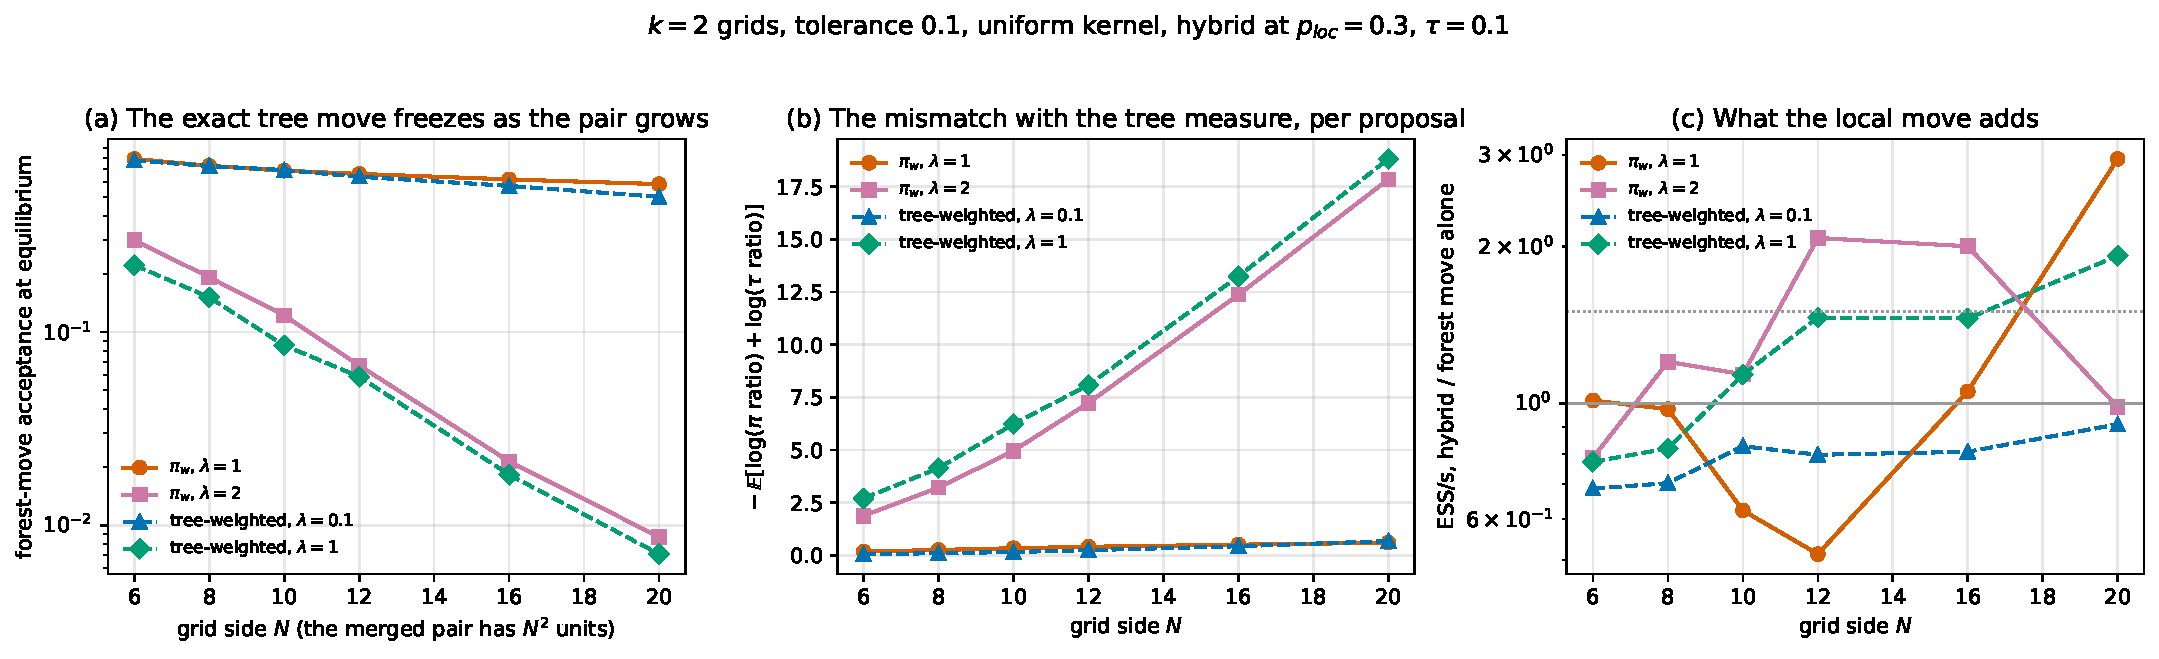
\includegraphics[width=\textwidth]{fig/forest_scaling.pdf}
  \caption{The exact tree move against grid side, $k = 2$,
    tolerance $0.1$, uniform kernel, hybrid at
    $p_{\mathrm{loc}} = 0.3$ and $\tau = 0.1$. (a)~Forest-move
    acceptance at equilibrium. (b)~Minus the mean of the target and
    tree-count log terms of \eqref{eq:forest-ratio} per feasible
    proposal, the per-proposal mismatch with the untempered tree
    measure. (c)~Effective samples per second of the hybrid over the
    forest move alone; the $N = 20$ points of the two tempered
    targets are not at equilibrium (see text).}
  \label{fig:scaling}
\end{figure}

\begin{table}[htbp]
\centering
\small
\begin{tabular}{lrrrrrr}
\toprule
 & $N = 6$ & 8 & 10 & 12 & 16 & 20 \\
\midrule
\multicolumn{7}{l}{\emph{forest-move acceptance at equilibrium}} \\
$\pi_w$, $\lambda{=}1$ & 0.79 & 0.73 & 0.69 & 0.66 & 0.62 & 0.58 \\
$\pi_w^{\mathrm{tree}}$, $\lambda{=}0.1$ & 0.78 & 0.73 & 0.69 & 0.64 & 0.57 & 0.50 \\
$\pi_w$, $\lambda{=}2$ & 0.30 & 0.19 & 0.12 & 0.067 & 0.021 & 0.009 \\
$\pi_w^{\mathrm{tree}}$, $\lambda{=}1$ & 0.22 & 0.15 & 0.085 & 0.059 & 0.018 & 0.007 \\
\multicolumn{7}{l}{\emph{mean cut length under the target}} \\
$\pi_w$, $\lambda{=}2$ & 7.2 & 10.0 & 12.6 & 15.1 & 19.8 & 25.1 \\
$\pi_w^{\mathrm{tree}}$, $\lambda{=}1$ & 6.9 & 9.7 & 12.1 & 15.0 & 20.0 & 25.1 \\
\multicolumn{7}{l}{\emph{per-proposal mismatch, $-\E[\log(\text{target ratio}) + \log(\text{tree-count ratio})]$}} \\
$\pi_w$, $\lambda{=}2$ & 1.9 & 3.2 & 5.0 & 7.2 & 12.4 & 17.9 \\
$\pi_w^{\mathrm{tree}}$, $\lambda{=}1$ & 2.7 & 4.2 & 6.2 & 8.1 & 13.2 & 18.8 \\
$\pi_w$, $\lambda{=}1$ & 0.2 & 0.3 & 0.3 & 0.4 & 0.5 & 0.6 \\
\multicolumn{7}{l}{\emph{local-move acceptance, $\tau = 0.1$ / $\tau = 0.03$}} \\
$\pi_w$, $\lambda{=}2$ & 0.39 / 0.74 & 0.32 / 0.69 & 0.25 / 0.63 & 0.19 / 0.59 & 0.12 / 0.49 & 0.08 / 0.42 \\
\multicolumn{7}{l}{\emph{ESS/s hybrid over forest, $\tau = 0.03$ (per step in parentheses)}} \\
$\pi_w$, $\lambda{=}2$ & 0.83 (0.78) & 1.03 (0.94) & 1.05 (0.91) & 1.86 (1.60) & 1.72 (1.46) & $[3.78]$ \\
$\pi_w^{\mathrm{tree}}$, $\lambda{=}1$ & 0.79 (0.76) & 0.89 (0.80) & 1.20 (1.03) & 1.53 (1.31) & 2.44 (2.11) & $[1.32]$ \\
\bottomrule
\end{tabular}
\caption{The scaling experiment. Acceptance, cut length and mismatch
  are from the hybrid's trace at $\tau = 0.1$; the local-move
  acceptance and the ratios are from the $\tau = 0.03$ rerun of the
  two tempered targets, which the move-size law calls for once the
  boundary grows. Bracketed ratios are at $N = 20$, where the forest
  move's effective sample size is $62$ and $77$ and the two chains'
  means differ by more than two standard errors, so neither chain is
  at equilibrium within the budget and the ratio is not a
  number.}\label{tab:scaling}
\end{table}

Three findings. First, the exact tree move freezes as the pair grows,
and the two tempered targets freeze it at the same rate. Under $\pi_w$
at $\lambda = 2$ and under $\pi_w^{\mathrm{tree}}$ at $\lambda = 1$
the forest move's acceptance falls on a straight line in log scale,
about $e^{-0.24 N}$, from $0.30$ and $0.22$ at $N = 6$ to $0.009$ and
$0.007$ at $N = 20$, while the per-proposal mismatch grows from about
$2$ to $19$ in proportion to the mean cut length ($7$ to $25$). The
two curves lie on top of each other in both panels of
Figure~\ref{fig:scaling}, although the tree-count term is present in
one Hastings ratio and absent from the other. What the move pays for
is the distance of the target from the untempered tree measure, not
the tree-count term as such. Under the two targets near that measure
the acceptance drifts from $0.8$ to $0.5$ over the same range and the
mismatch stays below one.

Second, the local move loses acceptance with pair size too, and has a
dial for it. At $\tau = 0.1$ its acceptance falls from $0.39$ to
$0.08$ between $N = 6$ and $20$, because its expected move
$2\tau|\partial_w|$ grows with the boundary and multi-unit draws are
more often infeasible. At $\tau = 0.03$ it is $0.74$ to $0.42$ over
the same range. The tree move has no such dial: its proposal is the
same law at every temperature and every kernel, so its acceptance is
set by the mismatch, which grows with the boundary.

Third, the local move's contribution grows with pair size where the
tree move pays. At $\tau = 0.03$ the hybrid's effective samples per
second relative to the forest move rise from below one at $N \le 10$
to $1.5$ to $2.4$ at $N = 12$ and $16$ for both tempered targets, with
the chains at the same level and the per-step ratios within $15$
percent of the per-second ones. At $N = 20$ neither chain reaches
equilibrium in $10^5$ steps under a tempered target, so that size is
beyond the budget of either chain and we do not quote a ratio. Under
the two near-proposal targets the ratio stays below one at every
size, as on Iowa under the tree-weighted target.

\textbf{What this establishes.} An exact tree move serves one family
of targets well, the mildly tempered tree measure, which is what
recombination samples anyway. For compactness targets away from it,
in either direction, its acceptance decays exponentially in the pair
size, and the diffusion move, whose ratio involves a one-unit boundary
change and whose reach is set by a timestep rather than by the
target, is the component that keeps an exact sampler moving. The Iowa
result of \S\ref{sec:exp-iowa} is one point on these curves, at a
pair size of about fifty units and a mismatch of about six.

\subsection{Iowa: the symmetric-\texorpdfstring{$q$}{q} filter against the exact sampler}\label{sec:exp-iowa-calib}

On Iowa there is no enumeration, but the exact chains of
\S\ref{sec:hybrid} estimate both targets directly, and the forest
move reaches the equilibrium of $\pi_w$ within about a thousand steps
where the partition-level tree move needed about $10^5$. Under the
uniform kernel at $\lambda = 0.1$ the forest move and the hybrid put
the nominal target's mean cut count at $88$ to $90$ (half-run means
$87.8$ to $90.1$ in Table~\ref{tab:iowa-short}) and the tree-weighted
tempered measure's at $41.0$ (half-run means $41.05$ and $40.93$).
Tempered ReCom with the symmetric-$q$ filter, run for 500 steps from
the same kind of tree-partition start (seed 42, burn-in 100, per-step
balance audit passed), sits at $39.8 \pm 4.3$ cuts, and Vanilla ReCom
at $41.4 \pm 4.8$; Chain E alone, climbing from the same start,
averages $55$ cuts over steps 100 to 500 and ends the run at $69$,
still rising. On real geography the chain practitioners run as
``targeting $\pi$'' therefore samples plans with less than half the
boundary length that $\pi$ itself has, and sits within one cut of the
tree-weighted tempered measure, with an exact sampler on each side of
the comparison. The $5 \times 5$ calibration showed the effect at the
level of distributions; Iowa shows its size.

\subsection{Precinct scale}\label{sec:exp-precinct}

\todo{To be written. North Carolina precinct dual graph (2\,692 units,
$k = 4$, $\varepsilon = 0.05$), perimeter and density targets, forest
move alone and hybrid at $p_{\mathrm{loc}} = 0.1$ with $\tau$ set by
the move-size rule, $2 \times 10^5$ steps, two seeds; a timing probe
first. Report forest acceptance, the two Hastings terms, quarter means,
ESS per step and per second, and the ratio. Expected from
\S\ref{sec:exp-scaling}: forest acceptance well below $10^{-2}$ under
the tempered targets at pairs of about 1\,300 units, hybrid reaching
equilibrium where the forest move alone does not.}

%════════════════════════════════════════════════════════════════════════════════
\section{Discussion}\label{sec:discussion}
%════════════════════════════════════════════════════════════════════════════════

\subsection{What each chain is for}\label{sec:disc-roles}

\textbf{Chain E} is provably exact for its target and, alone, too
immobile to be a sampler; its value is as the local component of the
hybrid. \textbf{The forest move} is the mobile exact component and
the baseline that practice runs; on its own measure, the mildly
tempered spanning-tree distribution, it is hard to improve on, and
away from it its acceptance decays with the pair size. \textbf{The
hybrid} is the practical exact sampler for kernel-weighted
compactness targets, with a small local fraction on real geography,
and a timestep set by the move-size law rather than fixed.
\textbf{The partition-level tree move} is kept as the move whose
closed form explains why Chain A is only approximate.
\textbf{Chains A and V} are what practitioners run, and
\S\ref{sec:exp-longrun} and \S\ref{sec:exp-iowa-calib} measure how
far their output sits from the tempered target and how close to the
tree-weighted one.

Why does the fidelity term matter? Without it the local move is a
fresh spectral re-split that discards the structure the chain has
found; with it the move is anchored and its size is governed by
Corollary~\ref{cor:small-tau}. The community step-trace diagnostic
(Appendix~\ref{sec:fiber-corridors}) makes a complementary point
about locality in general. Pure tree-move chains cross community
boundaries at 13--15\% per step, near the community-blind baseline,
while optimization-guided local mixtures drop to 5--11\%, which is
the division of labor the hybrid formalizes.

\subsection{Cost, and what a compiled implementation would change}\label{sec:disc-cost}

All chains here are Python. On Iowa under $\pi_w$ a forest step costs
about $1.1$\,ms (a Wilson draw, the balanced-edge scan, two
determinants and the crossing-edge sums, with the retry multiplying
the first), the partition-level tree move $0.18$\,ms, and a local step
about $1.5$\,ms, half of which is solver overhead on the pairs where
the balance window binds. A compiled forest step would be an order of
magnitude cheaper; the local step would gain less, since the solver
overhead is language independent. The per-second ratios of
\S\ref{sec:exp-iowa} would therefore move against the hybrid in Julia
or Rust, which is why every comparison also reports effective samples
per step. At $p_{\mathrm{loc}} = 0.1$ the per-step and per-second
ratios coincide on this implementation, so the headline result does
not depend on the language. Two improvements are within reach and
belong to the journal version: a closed-form solve for the local move
when the balance constraint is active (the unconstrained solve
shifted by a multiple of the population vector, one extra linear
solve and a scalar root), which removes the solver from the local
step entirely, and a per-pair timestep
$\tau = m / (2|\partial_w|)$ from Corollary~\ref{cor:small-tau} that
holds the expected move at $m$ units whatever the pair, the principled
form of the $\tau = 0.03$ rerun in \S\ref{sec:exp-scaling}.

\subsection{On the macro-structure findings}\label{sec:disc-throats}

The corrected picture of Appendix~\ref{sec:fiber-corridors} has two
consequences. First, it relocates the blame for slow local mixing. If
plan space were islands joined by narrow corridors, slow traversal
would be a topological inevitability; since the fibers are well
connected, it is a property of the dynamics, and \S\ref{sec:mobility}
identifies that property for Chain E as the feasibility of its draws,
not the graph. Second, worst-case hardness
results~\cite{akitaya2022reconfiguration,charikar2023complexity}
permit bottlenecked instances and Gold~\cite{gold2026adversarial}
exhibits planar-grid configurations that trap recombination for
exponentially many expected steps, so our grids may simply be too
small or too symmetric to show such structure; the statistics of
Table~\ref{tab:communities} give the template for checking a fiber
that does.

\subsection{Limitations}\label{sec:disc-limits}

\textbf{(L1) No theoretical mixing-time bound.} Like every
redistricting chain used in practice, we lack a polynomial
mixing-time guarantee (the polynomial-time grid sampler
of~\cite{cannon2024sampling} is not a local chain), and Chain E
demonstrates that even an exactly reversible chain can be an
extremely slow mixer. The scaling result is empirical, a straight
line over six grid sizes, with the independence-sampler argument of
\S\ref{sec:tree-pays} as its explanation and not its proof.

\textbf{(L2) Chain A's symmetric-$q$ approximation is not a small
bias.} On the enumerated fiber the tempered chain's empirical mean
($16.73$) sits $1.8$ cuts below the exact target mean ($18.56$), its
cut distribution is 220 noise-floor standard deviations from that
target (\S\ref{sec:exp-longrun}), and on Iowa the gap is a factor of
two in cut length (\S\ref{sec:exp-iowa-calib}).

\textbf{(L3) Chain E mixes too slowly to use alone.} Exactness comes
from single-shot rounding, whose reach Corollary~\ref{cor:small-tau}
bounds and whose feasibility \S\ref{sec:mobility} measures. Alone it
is not a sampler; in the hybrid it is a component whose value depends
on how far the target sits from the tree measure.

\textbf{(L4) The Iowa ratios carry about $25$ percent uncertainty and
rest on two seeds.} The forest move's effective sample size under
$\pi_w$ is in the hundreds at $2 \times 10^6$ steps. The direction,
the level agreement and the control are solid; the second decimal of
the ratio is not.

\textbf{(L5) Scale.} The largest real graph is 99 counties.
\S\ref{sec:exp-precinct} is to supply the precinct-scale run; until
then the scaling experiment on grids is the evidence that the effect
grows with pair size.

\subsection{Future directions}\label{sec:disc-future}

\begin{enumerate}
  \item The precinct-scale run of \S\ref{sec:exp-precinct}, and the
    downstream question it allows: whether the choice of kernel
    changes an ensemble's partisan statistics on real elections.
  \item The integer form of the energy, the same objective over
    $x \in \{0,1\}^{|V_H|}$ solved as a convex mixed-integer program
    inside a tempered chain, is an anchored refinement tool rather
    than a sampler. In an earlier version of this work we evaluated
    it as an optimizer on Iowa: it reduced mean cut edges by $20$
    percent over tempered ReCom, and simulated annealing over ReCom
    proposals reached the same best plans at a fraction of the cost.
    We record the result so that it need not be rediscovered, and do
    not pursue it.
  \item An informed marked-edge selection for the marked edge
    walk~\cite{mcwhorter2025marked}, with a Boltzmann draw over
    marked sets whose density is computable, would be the lifted-space
    analogue of Chain E; the same single-shot principle applies.
  \item Integration with the cycle walk~\cite{deford2025cycle} or the
    balanced up-down walk~\cite{akitaya2026bud} as the global
    component in place of the forest move, and multi-scale diffusion
    kernels in the local move.
\end{enumerate}

%════════════════════════════════════════════════════════════════════════════════
\section{Conclusion}\label{sec:conclusion}
%════════════════════════════════════════════════════════════════════════════════

This paper introduced a diffusion proposal for redistricting Markov
chains, one Laplacian energy
$\alpha\,x^\top L x + \beta\,\|x - x_0\|^2$ under global population
balance, and showed that the diffusion view is more than an
interpretation. The proposal is a single linear solve whenever
balance is slack, its expected move size is an explicit filter norm
with a small-timestep law and a hard ceiling, and its mobility is
governed by feasibility rather than by the Metropolis ratio.
Corrected by an exact Metropolis--Hastings step, the proposal gives
Chain E, to our knowledge the first optimization-based proposal in
redistricting MCMC with a detailed-balance argument, and on an
18-state fiber a million-step run's occupancy distribution is not
distinguishable from the exact target. Lifted to the spanning-forest
state space and mixed with the forest-lifted recombination move
Metropolized to the same target, it gives a reversible sampler for
kernel-weighted compactness targets, validated on 4\,006 enumerated
plans, that on Iowa roughly doubles the effective samples per second
of the forest move under perimeter and density targets and adds
nothing on the tree-weighted tempered measure. The reason is
structural and measured: an exact tree move proposes from the
untempered spanning-tree measure whatever the target, its acceptance
decays exponentially in the pair size under any compactness-tempered
target, and the local move has a dial for the same effect where the
tree move has none. On the enumerated $5 \times 5$ fiber we showed at
the level of distributions that tempered ReCom does not sample its
nominal target and sits close to the spanning-tree-weighted measure,
and on Iowa that the gap is a factor of two in boundary length.

For the field, we hope three ideas outlast the specific chains. Kernel
choice can be a first-class modeling decision inside the proposal and
the target rather than a post-hoc filter, provided the induced
distribution is corrected. The spanning-tree measure is the one
target a tree move samples for free, and every other target costs it
an acceptance that shrinks with the units in a pair, so a sampler for
compactness targets at precinct scale needs a move whose reach does
not depend on the target. And enumerated fibers are cheap, severe
test beds; a chain's distance from its own computable target on
4\,006 states, read against a noise floor, is a more informative
diagnostic than any p-value on a single trace.

\section*{Code and data availability}

All code, the enumerated fibers, and every artifact behind every table
and figure are in the public repository
\url{https://github.com/kirtisoglu/Redistricting_Diffusion_Model},
under \texttt{diffusion\_model/recom/}, with the scripts and command
lines listed in Appendix~\ref{app:reproducibility}. An archived
release with a persistent identifier will be deposited on acceptance.

%════════════════════════════════════════════════════════════════════════════════
\appendix
\section{Algorithm details and hyperparameters}\label{app:hyperparams}
%════════════════════════════════════════════════════════════════════════════════

\subsection{Common setup}\label{app:common}

\begin{itemize}
  \item Dual graph $G = (V, E)$ with vertex populations $p_v$ and
    edge attributes (\texttt{shared\_perim} for Iowa).
  \item $k$ districts, $\varepsilon$-population balance per
    Equation~\eqref{eq:pop-balance}, enforced as a two-sided bound around the
    global ideal on every move (Equation~\eqref{eq:balance-window})
    and audited per step. The bare GerryChain \texttt{recom} proposal
    is wrapped with an explicit whole-plan balance check
    (\texttt{recom\_valid}), since its internal cut search validates
    only one side of each split.
  \item Initial partition from
    \texttt{gerrychain.tree.recursive\_tree\_part}, redrawn until all
    $k$ districts satisfy the global tolerance
    (\texttt{balanced\_tree\_part}); vertical split for the $k = 2$
    grids.
  \item Step counts: $5 \times 5$ baselines $N = 1\,000$, burn-in
    $100$; Iowa baselines $N = 500$, burn-in $100$; long-run
    validation (\S\ref{sec:exp-longrun}) $2 \times 10^5$ (A) and
    $10^5$ (E); $5 \times 5$ forest-move validation
    (\S\ref{sec:exp-hybrid}) $2 \times 10^5$; Iowa short runs
    $2 \times 10^5$, long runs $2 \times 10^6$ under $\pi_w$ and
    $5 \times 10^5$ under $\pi_w^{\mathrm{tree}}$; scaling experiment
    $5 \times 10^4$ per chain, $10^5$ for $N \ge 16$. Burn-in $10\%$
    unless stated.
  \item Random seeds: base seed 42 with a distinct offset per chain
    (independent streams for Python \texttt{random} and
    \texttt{numpy}); seed 43 for the second Iowa long run.
\end{itemize}

\subsection{Chain-specific parameters}\label{app:chains}

Table~\ref{tab:hyperparams} lists every locked value.

\begin{table}[htbp]
\centering
\small
\begin{tabular}{lll}
\toprule
Chain & Parameter & Value \\
\midrule
A & $\lambda$ (target temperature) & 0.10 \\
E & $\alpha$, $\beta$ & 1.0, 10.0 ($\tau = \alpha/\beta = 0.1$) \\
E & Rounding & single-shot Bernoulli($x^\star$), clip $10^{-12}$ \\
T & cut edge & uniform over all tree edges; fair-coin labels \\
F & cut edge & uniform over balanced tree edges; fair-coin labels; retry up to 20 trees \\
F & pair & uniform over boundary pairs \\
H & $p_{\mathrm{loc}}$ & 0.1 (Iowa long runs), 0.1 and 0.3 (Iowa short runs), 0.2 ($5 \times 5$), 0.3 (grids) \\
H & $\tau$ & 0.1; 0.03 in the rerun of \S\ref{sec:exp-scaling} \\
Iowa $\lambda$ & uniform / perimeter / density & 0.100 / 0.343 / 0.718 (equal tempering at the start plan) \\
\bottomrule
\end{tabular}
\caption{Locked-in hyperparameters for the chains of
  Table~\ref{tab:chains}.}\label{tab:hyperparams}
\end{table}

\subsection{Compute environment}\label{app:compute}

\begin{itemize}
  \item macOS (Darwin 23.6.0), Python 3.12, and a Linux container
    (Python 3.13) for the analytic checks and prototypes.
  \item Gurobi 13.0 (academic license) for the QP solves that the
    linear-solve path of Lemma~\ref{lem:row-stochastic} does not
    cover.
  \item GerryChain 0.2.22 for the ReCom proposal and the initial tree
    partitions; NetworkX 3.x for graph operations.
  \item One Python process per chain, single-threaded, at reduced
    priority; the ten Iowa long runs and the scaling chains ran
    concurrently on an 11-core machine, each forest chain at the same
    time as its hybrid partner so that both members of a ratio see
    the same load. All ratios are also reported per step.
\end{itemize}

%════════════════════════════════════════════════════════════════════════════════
\section{Partition fiber structure: communities without bottlenecks}\label{sec:fiber-corridors}

This appendix documents a structural diagnostic of the partition fiber
$\mathcal{P}_k(G; \varepsilon)$ (the set of all valid plans), viewed as a graph under its minimal
valid move relation. Two findings emerge, one positive and one
negative, and we report both. Positively, all three enumerated fibers
carry genuine mesoscale community structure, with modularity far above
degree-preserving null models, and chains differ sharply in how often
they cross community boundaries. Negatively, a plausible folk
intuition (that the communities are ``islands'' joined by narrow
corridors or bottleneck edges) is refuted by method-independent
statistics. Community interfaces are wide, nearly all community pairs
are directly connected, and the literal bridges of the exact-balance
fiber turn out to be pendant vertices. The diagnostic still motivates
the local-refinement design of \S\ref{sec:model}, and we believe both
findings are of independent interest for analyzing redistricting
MCMC.

\paragraph{Three test beds.}\label{sec:fiber-testbeds}

We construct three fully enumerated partition fibers spanning grid
size, district count, and balance tolerance (Table~\ref{tab:fibers}).

\begin{table}[htbp]
\centering
\small
\begin{tabular}{lrrrrrl}
\toprule
Fiber & Nodes & Edges & $k$ & $\varepsilon$ & Sizes & Adjacency \\
\midrule
$5 \times 5$, $\varepsilon = 0$    & 4\,006   & 13\,416  & 5 & 0    & \{5\}       & boundary swap \\
$5 \times 5$, $\varepsilon = 0.20$ & 193\,128 & 969\,760 & 5 & 0.20 & \{4, 5, 6\} & single flip \\
$4 \times 4$, $\varepsilon = 0.25$ & 1\,953   & 7\,024   & 4 & 0.25 & \{3, 4, 5\} & single flip \\
\bottomrule
\end{tabular}
\caption{The three test-bed fibers. Adjacency is the \emph{minimal
  valid move} of each fiber. At $\varepsilon = 0$ no single-vertex
  reassignment preserves exact balance (it produces districts of sizes
  4 and 6), so adjacency is the boundary \emph{swap}, which exchanges one
  boundary vertex of district $a$ with one of district $b$, both
  districts remaining connected. At $\varepsilon > 0$ adjacency is the
  single \emph{flip}, which reassigns one boundary vertex, both affected
  districts remaining connected and within size bounds. Cross-fiber
  comparisons carry one caveat. The $\varepsilon = 0$
  fiber lives under a different (two-vertex) move relation than the
  $\varepsilon > 0$ fibers.}\label{tab:fibers}
\end{table}

For each fiber, all valid partitions are enumerated and the single-flip
adjacency graph is built explicitly (enumeration runtimes on a 2024
MacBook range from $\sim 5$ s for the $4 \times 4$,
$\varepsilon = 0.25$ fiber to $\sim 50$ min for the $5 \times 5$,
$\varepsilon = 0.20$ fiber; scripts accompany the replication
materials).

\paragraph{Community structure, validated against null models.}\label{sec:fiber-islands}

Each fiber graph carries substantial mesoscale community structure
under modularity maximization. We report the method per fiber (greedy
modularity, Clauset--Newman--Moore, for the $\varepsilon = 0$ and
$4 \times 4$ fibers; Louvain, resolution $1.0$, seed 42, for the large
$\varepsilon = 0.20$ fiber), validate against degree-preserving
rewiring nulls, and treat the specific community counts as
method-dependent descriptive statistics.

\begin{table}[htbp]
\centering
\small
\begin{tabular}{lrrrlrrr}
\toprule
& \multicolumn{4}{c}{Community structure}
& \multicolumn{3}{c}{Anti-bottleneck statistics} \\
\cmidrule(lr){2-5}\cmidrule(lr){6-8}
Fiber & Comm. & $Q$ & Null $Q$ & Method
      & Pairs conn. & Inter-comm.\ edges & Width (med/max) \\
\midrule
$5 \times 5$, $\varepsilon = 0$    & 10 & 0.65 & 0.36 & CNM
  & 15/15 & 18.3\% & 142 / 383 \\
$5 \times 5$, $\varepsilon = 0.20$ & 26 & 0.69 & n/a  & Louvain
  & 320/325 & 26.8\% & 667 / 3\,006 \\
$4 \times 4$, $\varepsilon = 0.25$ & 7  & 0.58 & 0.34 & CNM
  & 21/21 & 23.3\% & 71 / 186 \\
\bottomrule
\end{tabular}
\caption{Left: community decompositions with degree-preserving null
  baselines (mean $Q$ of CNM on double-edge-swap rewirings of the same
  graph; the $193$k-node fiber's null is omitted for cost). Real $Q$
  exceeds null $Q$ by $0.24$--$0.29$, so the community structure is
  genuine, not a degree-sequence artifact. Counts vary with the
  detection method and should be read qualitatively. Right:
  the statistics that refute the corridor picture. Nearly every pair
  of communities shares a direct interface (``pairs conn.''\ counts
  the large-community pairs at $\varepsilon = 0$), interfaces are
  tens to thousands of edges wide, and a fifth to a quarter of all
  fiber edges run between communities. The exact-balance fiber's 16
  literal single-edge bridges each split off a \emph{single vertex}
  (pendant leaves), not an island, and the six large
  $\varepsilon = 0$ communities have conductance $0.15$--$0.22$, an
  order of magnitude above bottleneck territory.}
\label{tab:communities}
\end{table}

\paragraph{No narrow corridors: a corrected intuition.}\label{sec:fiber-corridors-invariant}

It is tempting to picture these communities as islands joined by a few
narrow corridors, with bottleneck edges controlling passage. The
method-independent statistics on the right of
Table~\ref{tab:communities} refute that picture on all three
fibers.

Concretely, on the $\varepsilon = 0.20$ fiber, interfaces thinner than
50 edges do exist (there are 16 of them), but they are simply the tail
of a width distribution whose median is 667 and whose top interfaces
carry $3\,000$ edges; a chain moving through this graph crosses
between communities through the wide interfaces, and the thin tail is
irrelevant to mixing. The correct summary of fiber macro-structure is
therefore \emph{communities without bottlenecks}. Valid-plan space is
regionally organized but well connected, and slow traversal by local
chains (below) is a property of the \emph{dynamics}, not of corridor
topology. This negative result matters for chain design. It says
local chains stall not because the state space is nearly disconnected
but because their moves are small and, in Chain E's case, because
distant proposals are rarely feasible (\S\ref{sec:mobility}); global
recombination moves, by
contrast, relocate across communities in a single step.

\paragraph{Chain step-trace diagnostic.}\label{sec:fiber-trace}

The community decomposition supports a direct diagnostic for any
redistricting chain. We label each visited partition by its
greedy-modularity community on the $\varepsilon = 0$ fiber and record
the \emph{jump rate}, the fraction of steps that move to a
different community (Table~\ref{tab:island-trace}).

\begin{table}[htbp]
\centering
\small
\begin{tabular}{lrrr}
\toprule
Chain & Communities visited & Jump rate & Jumps in 1\,000 steps \\
\midrule
V: Vanilla ReCom        & 8/10 & 15.3\% & 153 \\
A: Tempered ReCom       & 7/10 & 12.7\% & 127 \\
B: ReCom + continuous QP, deterministic rounding (50/50) & 6/10 & 4.6\%  & 46  \\
C: Tempered ReCom + integer QP refinement    & 6/10 & 10.5\% & 105 \\
D: ReCom + spectral mix & 7/10 & 9.3\%  & 93  \\
E: QP-MH exact          & 2/10 & 0.3\%  & 3   \\
\bottomrule
\end{tabular}
\caption{Inter-community jump rates on the $5 \times 5$,
  $\varepsilon = 0$ fiber (1\,000 steps per chain, seed 42, per-chain
  RNG streams). A community-blind baseline crosses at roughly the
  inter-community edge share (18.3\%,
  Table~\ref{tab:communities}); ReCom variants (V, A) sit near it
  at $\sim 13$--15\% per step, the local kernels (B, C, D) are
  stickier at $\sim 5$--11\%, and the strictly local QP-MH chain (E)
  almost never crosses, a property of its small accepted moves rather
  than of any bottleneck in the fiber. Chains B, C and D are the
  deterministic-rounding mixtures of an earlier version of this work
  (\S\ref{sec:rounding}, \S\ref{sec:disc-future}), included because
  the diagnostic was run on all six.}\label{tab:island-trace}
\end{table}

\textbf{Reading of the diagnostic.} ReCom relocates across
communities in single steps; optimization-guided local kernels work
within them; and the exact-but-strictly-local Chain E shows the
failure mode of small accepted moves. The regimes are complementary,
and they suggest an explicit design principle. A good redistricting
sampler should combine global moves that relocate across regions of
plan space with local moves that refine within them; the forest move
does the former, the anchored local kernel the latter. This is the
design of the hybrid of \S\ref{sec:hybrid}, each step a random mixture
of a tree move and a diffusion move. We note the diagnostic's limits
(one run per chain on one fiber, and community labels from a specific
detection method) and read it as motivating evidence, not proof.

%════════════════════════════════════════════════════════════════════════════════
\section{Reproducibility checklist}\label{app:reproducibility}
%════════════════════════════════════════════════════════════════════════════════

\begin{itemize}
  \item Code: \texttt{diffusion\_model/recom/} in the project
    repository.
  \item Modules: \texttt{problems.py} (graph setup, balanced initial
    plans), \texttt{chains.py} (chain runners, balance-validated
    ReCom wrapper, per-step audit), \texttt{qp\_model.py}
    (QP and QP-MH step factories, global-ideal balance windows),
    \texttt{hybrid.py} (the partition-level tree move, Chain E with
    the linear-solve path, and their analytic check),
    \texttt{forest\_recom.py} (the forest move, the lifted local move,
    the two targets, and the analytic check on the lifted
    $2 \times 3$ fiber), \texttt{kill\_stats.py} (ESS, noise floors,
    batch-means Hotelling with bin merging), \texttt{diagnostics.py}.
  \item Orchestrators: \texttt{iowa\_target\_matched.py} (the
    baseline chains V, A and E), \texttt{long\_run\_5x5.py} and
    \texttt{matrix\_tree\_targets.py} (\S\ref{sec:exp-5x5}),
    \texttt{calibration\_distance.py} and \texttt{fig\_calibration.py}
    (\S\ref{sec:exp-longrun}), \texttt{db\_check\_2x3.py}
    (Remark~\ref{rem:qpmh-scope}), \texttt{long\_run\_2x3.py} with
    \texttt{gof\_2x3.py} (\S\ref{sec:exp-2x3}; arguments
    \texttt{1000000 42}), \texttt{spectral\_move\_size.py} and
    \texttt{fig\_spectral.py} (\S\ref{sec:diffusion-theory}),
    \texttt{acceptance\_sweep.py} (Table~\ref{tab:mobility}),
    \texttt{mobility\_law.py} (Table~\ref{tab:mobility-law}),
    \texttt{forest\_validate\_5x5.py} (Table~\ref{tab:hybrid-5x5};
    arguments \texttt{200000 42 0.2 0.1 pi} and \texttt{... tree}),
    \texttt{forest\_iowa.py} (Tables~\ref{tab:iowa-short}
    and~\ref{tab:iowa-long}; \texttt{short 200000 42 0.1 pi|tree},
    \texttt{long forest|hybrid 2000000 42|43 pi [0.3]},
    \texttt{long forest|hybrid 500000 42|43 tree}),
    \texttt{forest\_verdict.py} (the verdict table),
    \texttt{forest\_scaling.py} with \texttt{forest\_scaling\_parallel.py}
    (Table~\ref{tab:scaling}, Figure~\ref{fig:scaling}; arguments
    \texttt{50000 42 6,8,10,12,16,20 pi:1,pi:2,tree:0.1,tree:1 0.3
    --fig}, and the same with \texttt{TAU = 0.03} for the rerun),
    \texttt{hybrid\_validate\_5x5.py}, \texttt{hybrid\_iowa.py} and
    \texttt{hybrid\_iowa\_long.py} (the partition-level tree move's
    rows), \texttt{ten\_seed\_stats.py} (between-seed statistics).
  \item Outputs, all under \texttt{iowa\_hybrid\_test\_out/}, each
    stamped with its configuration: \texttt{target\_matched\_*.npz},
    \texttt{long\_run\_5x5\_seed42.npz}, \texttt{matrix\_tree\_targets.npz},
    \texttt{calibration\_distance\_seed42.npz},
    \texttt{long\_run\_2x3\_n*\_seed42.npz},
    \texttt{spectral\_move\_size.npz}, \texttt{acceptance\_sweep\_5x5.npz},
    \texttt{mobility\_law\_5x5.npz}, \texttt{hybrid\_*.npz},
    \texttt{forest\_validate\_5x5\_*.npz}, \texttt{forest\_iowa\_*.npz},
    \texttt{forest\_verdict.txt}, \texttt{forest\_scaling\_seed42*.npz},
    with the console logs beside them.
  \item Fibers: \texttt{fiber\_5x5/} contains the $5 \times 5$ and
    $4 \times 4$ enumeration scripts and precomputed
    adjacency files.
  \item Reproducibility across sessions. The $5 \times 5$ runs and the
    Iowa runs under the uniform and density kernels reproduce bit for
    bit from their seeds. The Iowa runs under the perimeter kernel do
    not: a repeat of one $\tau = 0.1$ session matched the stored
    trajectories for 21\,217 and 185\,390 steps and then diverged,
    which we attribute to floating-point sensitivity of the QP solver
    fallback under that kernel's wide range of edge weights. The
    stored artifacts are the realizations reported, and every
    perimeter-target conclusion rests on long runs and two seeds.
  \item Precinct scale: \todo{data file, commands and artifacts of
    \S\ref{sec:exp-precinct}.}
\end{itemize}

\bibliographystyle{plain}
\bibliography{ref}

\end{document}
